\begin{enumerate}[label=\thesubsection.\arabic*, ref=\thesubsection.\theenumi]
	%---------------------Q1-----------------
	\item Find the value of $x$ ,if $\myvec{3x+y & -y \\
										2y-x  & 3}    = \myvec{1 & 2 \\
										                       -5 & 3  }$\\
    \solution 
    Since both Matrices are equal their difference is equal to Null matrix
    \begin{align}
    	\myvec{3x+y & -y \\
    	        2y-x & 3}  - \myvec{1 & 2 \\
    	                             -5 & 3} =\myvec{0 & 0 \\
    	                                             0 & 0 } \\
    	\myvec{3x+y-1 & -y-2 \\
    	       2y-x+5 &  0} = \myvec{0 & 0 \\
    	                             0 & 0 } \\
    	                              \end{align}
    	                              
    	Since it's a Null matrix,each element equal's 0
    	\begin{align}
    	i.e,        3x+y-1=0,-y-2=0,2y-x+5=0 \\
    \end{align}
    solving above eqations we get
    \begin{align}
    	x=1 , y=-2
    \end{align}
	%--------------------------------q2---------------------
   
   %===============================Q3=========================
   
   \item Evaluate:     $$\int \frac{\sec^2(\sqrt{x})}{\sqrt{x}} \, dx$$
   \solution
   Let:
   \begin{align}
   x = t^2 \quad \implies \quad \sqrt{x} = t \quad (\text{for } t > 0)
   \end{align}
   Differentiating both sides with respect to $t$:
   \begin{align}
   	dx = 2t \, dt
   	\end{align}
   	
   	Substitute equations \brak{1.2.3.1} and \brak{1.2.3.2} into the original integral:
   \begin{align}
	I &= \int \frac{\sec^2(\sqrt{x})}{\sqrt{x}} \, dx \\
	&= \int \frac{\sec^2(t)}{t} \cdot (2t \, dt) \\
	&= \int \sec^2(t) \cdot \frac{2t}{t} \, dt \\
	&= 2 \int \sec^2(t) \, dt
   	\end{align}
   	 From \eqref{eq:tandiff}
   	\begin{align}
   		I = 2 \tan(t) + C
   		\end{align}
   	From \eqref{euler_met}
   		\begin{figure}[htbp] % [htbp] specifies preferred placement (here, top, bottom, page)
   			\centering
   			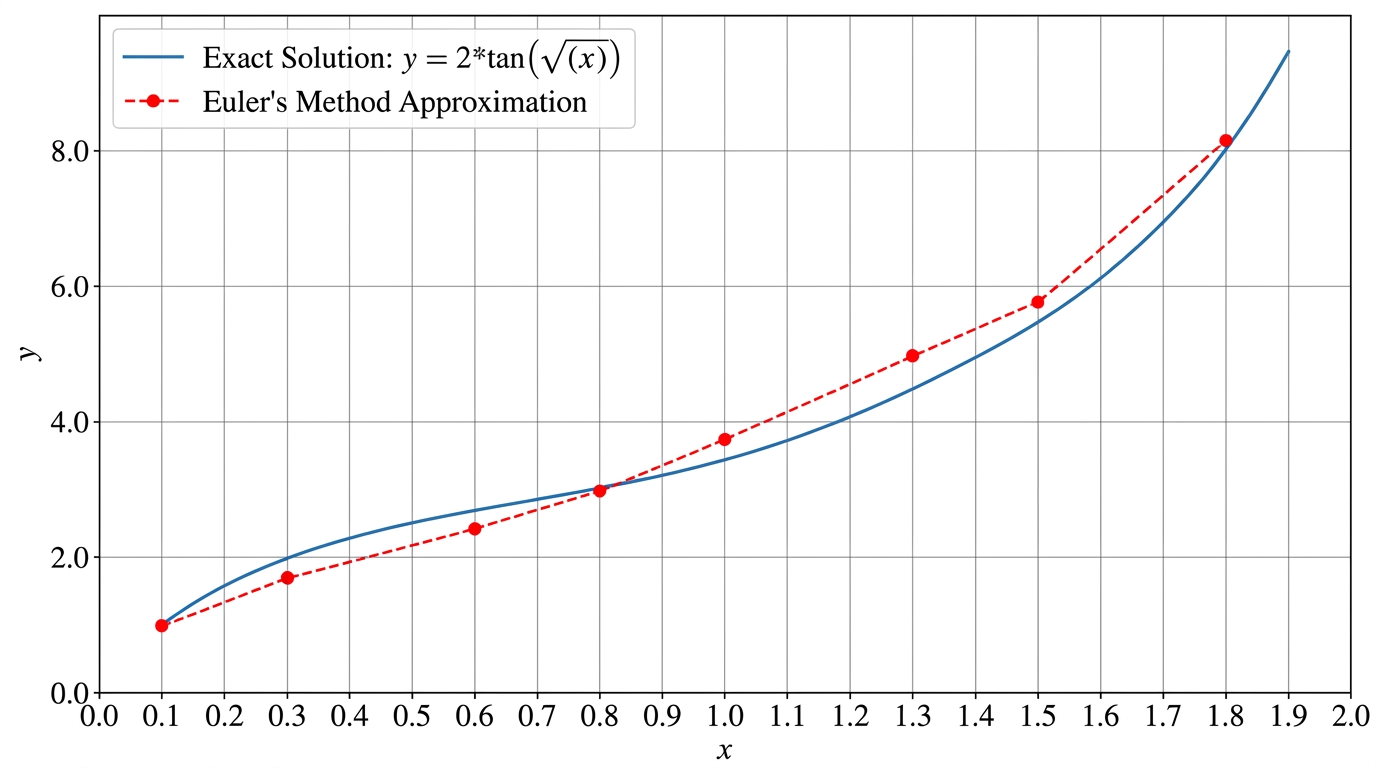
\includegraphics[width=0.6\textwidth]{figs/q2}
   			\caption{Euler method vs Exact solution}
   			\label{euler_fig1}
   		\end{figure} \newpage
   		\begin{lstlisting}
   			/codes/q2.py
   		\end{lstlisting}
   %==============================Q4=======================================
   \item Evaluate:
   $$\int \frac{\cos x}{\sqrt{1 + \sin x}} \, dx$$
   \solution
   
   Let:
   \begin{align}
	u = 1 + \sin x
   	\end{align}
   	Differentiating both sides with respect to $x$,
   	From \eqref{eq:sindif}
   	\begin{align}
   		\frac{du}{dx} = \cos x \quad \implies \quad du = \cos x \, dx
   	\end{align}
   	Substitute $u$ and $du$ into the original integral $I_2$:
   	\begin{align}
   		I_2 &= \int \frac{\cos x \, dx}{\sqrt{1 + \sin x}} \\
   		&= \int \frac{du}{\sqrt{u}} \\
   		&= \int u^{-1/2} \, du\\
   		I_2 &= \frac{u^{-1/2 + 1}}{-\frac{1}{2} + 1} + C_2 \\
   		&= \frac{u^{1/2}}{\frac{1}{2}} + C_2 
   		\end{align}
   		\begin{align}
   			&= 2 \sqrt{u} + C_2
   	\end{align}
   	 Replacing $u$ with $1 + \sin x$:
   	\begin{align}
   		I_2 = 2 \sqrt{1 + \sin x} + C_2
   	\end{align}
   		From \eqref{euler_met}
   	\begin{figure}[htbp] % [htbp] specifies preferred placement (here, top, bottom, page)
   		\centering
   		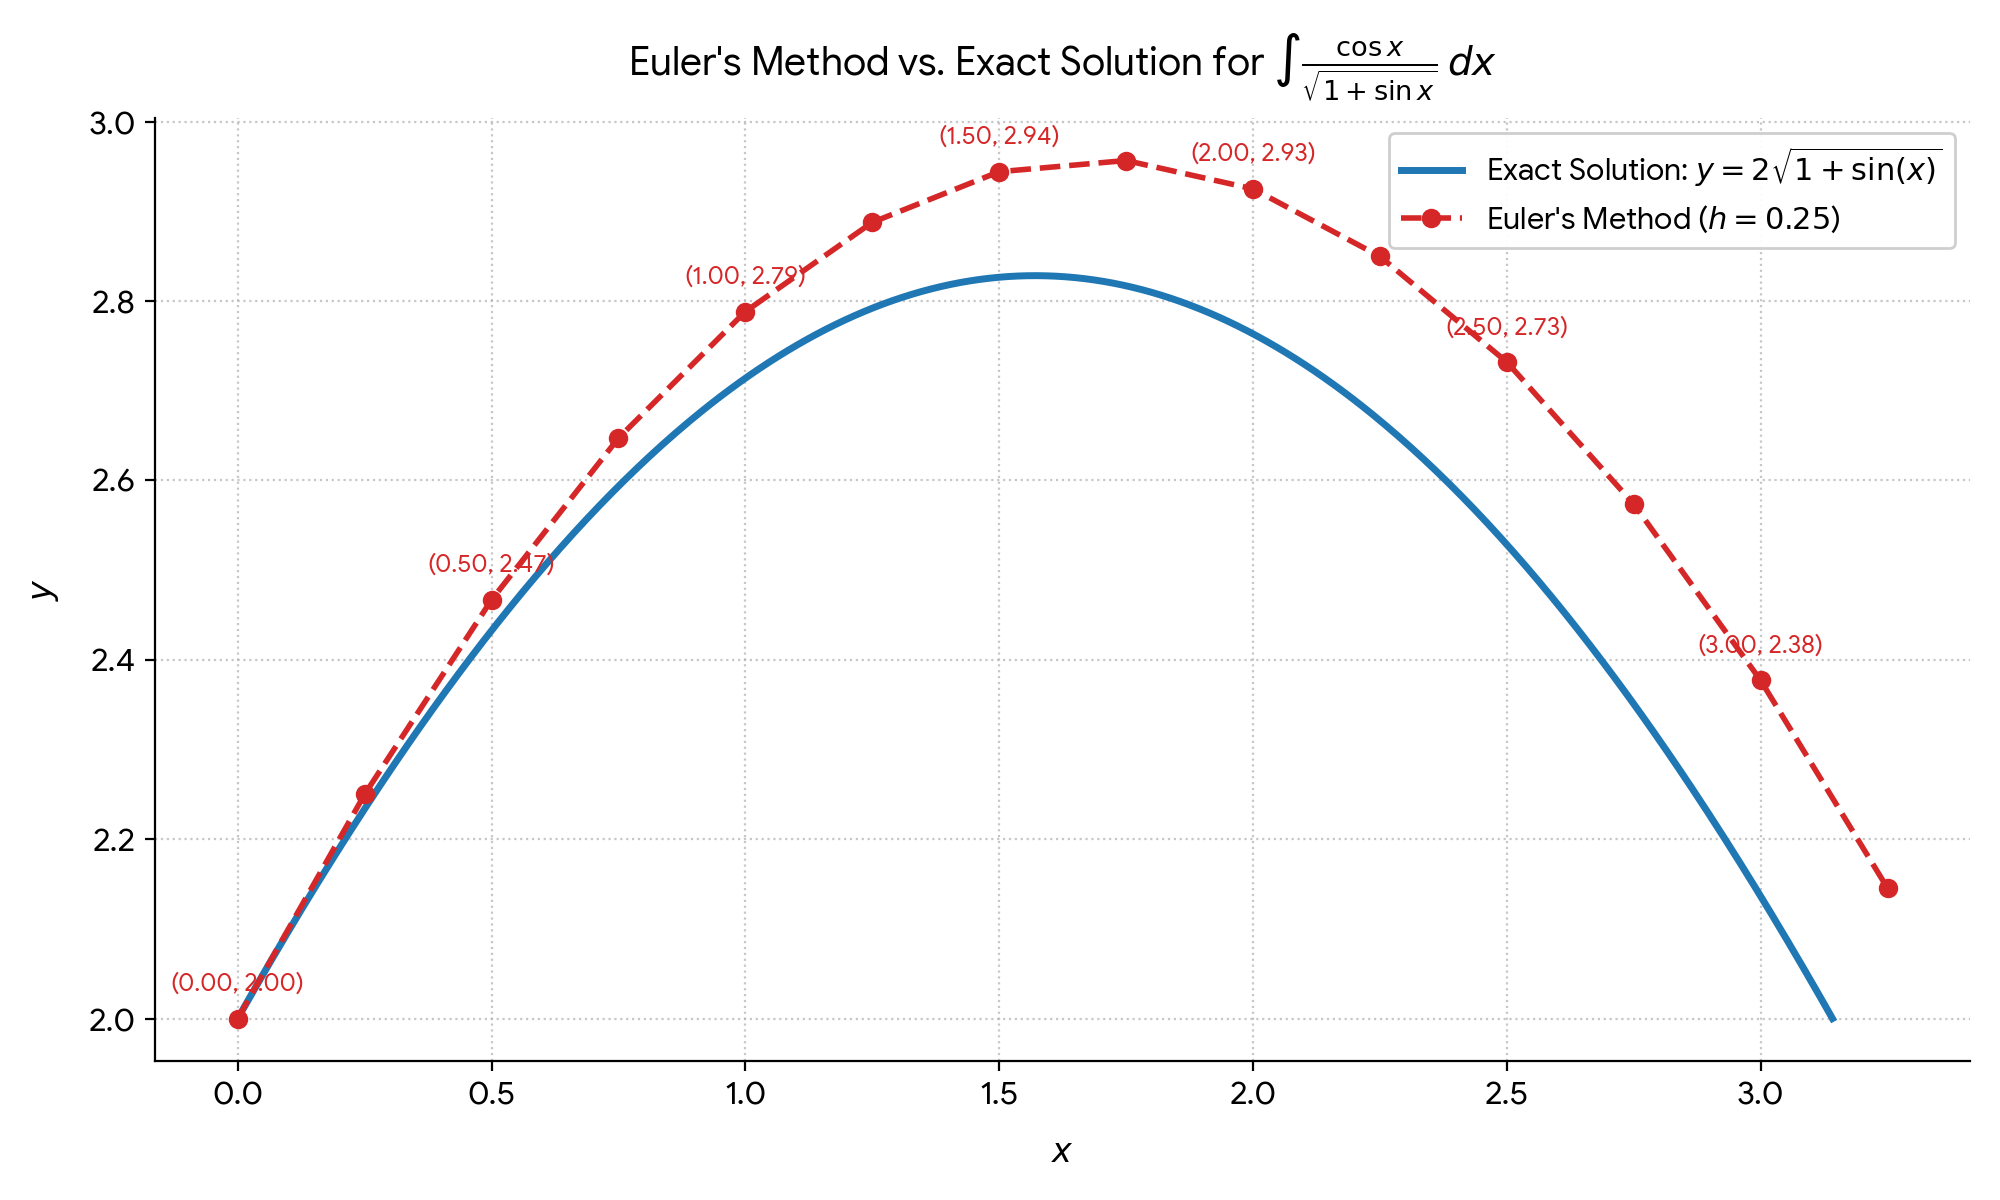
\includegraphics[width=0.6\textwidth]{figs/q3}
   		\caption{Euler method vs Exact solution}
   		\label{euler_fig2}
   	\end{figure} 
   	\begin{lstlisting}
   		/codes/q3.py
   	\end{lstlisting}
   	
   %==========================Q5========================================
   \item Write the principal value of $\cos^{-1}\brak{\cos \frac{7\pi}{6}}$ \\
  \solution 
  From \eqref{eq:inverse}
  \begin{align}
  	\cos^{-1}(\cos(x)) = 2\pi - x = 2\pi - \frac{7\pi}{6} = \frac{5\pi}{6}
  	\end{align}
  	\begin{figure}[htbp] % [htbp] specifies preferred placement (here, top, bottom, page)
  	\centering
  	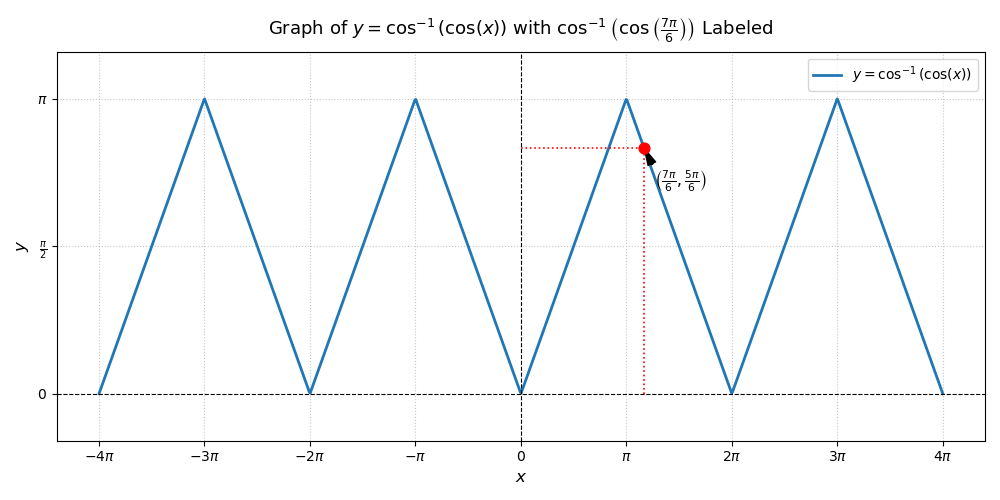
\includegraphics[width=0.5\textwidth]{figs/Fig_1}
  	\caption{Graph of  $\cos^{-1}\brak{\cos x}$. }
  	\label{fig:my_image}
  	\end{figure}
  	\begin{lstlisting}
  		/codes/q4.py
  		\end{lstlisting}
   
   
   
   
   
   
   
   %===========================Q6=================================
   \item Write the value of the following determinant:
   \begin{align*} 
   		\mydet {a-b & b-c & c-a \\
                b-c & c-a & a-b \\
                c-a & a-b & b-a }
    \end{align*}
    \solution 
    \begin{align}
    	\mydet {a-b & b-c & c-a \\
    		b-c & c-a & a-b \\
    		c-a & a-b & b-a } \xrightarrow{R_1 \to R_1+R_2+R_3}\mydet{0 & 0 & 0 \\
    		                                                          b-c & c-a & a-b \\ c-a & a-b & b-a}=0 
    \end{align}		
    All elements of any row of a determinant are zero, the value of the determinant is 0.
    \begin{align}
    \mydet {a-b & b-c & c-a \\
    	b-c & c-a & a-b \\
    	c-a & a-b & b-a }=0
    \end{align}
    
    
    %==================================Q7===========================                                                           
    \item Find the value of $x$ from the following:
     \begin{align*}
     \mydet{a+x & a-x & a-x \\
       a-x & a+x & a-x \\
        a-x & a-x & a+x }  = 0
     \end{align*} 
     \solution
          
    \begin{align}
    	\mydet{a+x & a-x & a-x \\
    		a-x & a+x & a-x \\
    		a-x & a-x & a+x }  = 0  \xrightarrow{R_1 \to R_1+R_2+R_3}
    	\mydet{3a-x & 3a-x & 3a-x \\
    		a-x & a+x & a-x \\
    		a-x & a-x & a+x} = 0
    \end{align}
    Factoring out $\brak{3a-x}$ from the first row $R_1$,
    \begin{align}
    	\brak{3a-x} \mydet{1 & 1 & 1 \\
    		a-x & a+x & a-x \\
    		a-x & a-x & a+x} = 0  \xrightarrow[R_3 \to R_3 - \brak{a-x}R_1] {R_2 \to R_2 - \brak{a-x}R_1 } 
    	\brak{3a-x} \mydet{1 & 1 & 1 \\
    		0 & 2x & 0 \\
    		0 & 0 & 2x} = 0
    \end{align}
    Since the matrix is upper triangular, evaluating its determinant as the product of its diagonal elements yields:
    \begin{align}
    	\brak{3a-x} \cdot \brak{1 \cdot 2x \cdot 2x} &= 0
    	\\
    	4x^2 \brak{3a-x} &= 0
    \end{align}
    giving the roots
    \begin{align}
    	x = 0 , x = 3a
    \end{align}
                    
    %===============================Q8============================
    \item Find the value of $p$ if: $$(2\vec{e}_1 + 6\vec{e}_2 + 27\vec{e}_3) \times (\vec{e}_1 + 3\vec{e}_2 + p\vec{e}_3) = \vec{0}$$
    \solution
   Let:
   \begin{align}
   	\vec{w} = \myvec{2 \\ 6 \\ 27}, \quad \vec{v} = \myvec{1 \\ 3 \\ p}
   \end{align}
   From \eqref{eq:cross}
   \begin{align}
     \myvec{6p - 27\brak{3} \\ 27\brak{1} - 2p \\ 2\brak{3} - 6\brak{1}} = \myvec{6p - 81 \\ 27 - 2p \\ 0}=\vec{0}
    \end{align}
    \begin{align}
    	6p - 81 = 0 &\implies p = \frac{27}{2}
    	\\
    	27 - 2p = 0 &\implies p = \frac{27}{2}
    \end{align}
    Thus, the required value of $p$ is $\frac{27}{2}$.
    %==============================Q9====================================================
    \item Write the direction cosines of a line equally inclined to the three coordinate axes.
    \solution
    As they are equally inclined to all the axes ($\alpha = \beta = \gamma$)
    From \eqref{eq:cross}
    \begin{align}
    	l = m = n = k
    \end{align}
    Expressing $\vec{u}$ in terms of $k$ and the vector of ones $\vec{1} = \myvec{1 \\ 1 \\ 1}$,
    \begin{align}
    	\vec{u} = k \vec{1} = k \myvec{1 \\ 1 \\ 1}
    \end{align}
    Using the unit norm condition $\norm{\vec{u}}^2 = \vec{u}^{\top} \vec{u} = 1$:
    \begin{align}
    	\brak{k \vec{1}}^{\top} \brak{k \vec{1}} &= 1
    	\\
    	k^2 \myvec{1 & 1 & 1} \myvec{1 \\ 1 \\ 1} &= 1
    	\\
    	3k^2 &= 1 \implies k = \pm \frac{1}{\sqrt{3}}
    \end{align}
    Therefore, the direction cosines of the line are
    \begin{align}
    	\myvec{l \\ m \\ n} = \pm \myvec{\frac{1}{\sqrt{3}} \\ \frac{1}{\sqrt{3}} \\ \frac{1}{\sqrt{3}}}
    \end{align}
    %===========================Q10===========
    \item If $\vec{p}$ is a unit vector and $\brak{\vec{x} - \vec{p}} \cdot \brak{\vec{x} + \vec{p}} = 80$, then find \mydet{\vec{x}}.
    \solution
    As
    \begin{align}
    	\norm{\vec{p}} = 1 \implies \vec{p}^{\top}\vec{p} = 1
    \end{align}
  	
    \begin{align}
    	\brak{\vec{x} - \vec{p}} \cdot \brak{\vec{x} + \vec{p}} = 80
    	&\implies
    	\brak{\vec{x} - \vec{p}}^{\top} \brak{\vec{x} + \vec{p}} = 80
    	\\
    	\vec{x}^{\top}\vec{x} + \vec{x}^{\top}\vec{p} - \vec{p}^{\top}\vec{x} - \vec{p}^{\top}\vec{p} &= 80
    \end{align}
    As vector dot product is commutative ($\vec{x}^{\top}\vec{p} = \vec{p}^{\top}\vec{x}$)
    \begin{align}
    	\norm{\vec{x}}^2 - \norm{\vec{p}}^2 &= 80
    	\\
    	\norm{\vec{x}}^2 - 1 &= 80
    	\\
    	\norm{\vec{x}}^2 &= 81
    	\\
    	\implies \norm{\vec{x}} &= 9
    \end{align}
    
    %===========================Q11===========
    \item The length $x$ of a rectangle is decreasing at the rate of $5 \text{ cm/minute}$ and the width $y$ is increasing at the rate of $4 \text{ cm/minute}$. When $x = 8 \text{ cm}$ and $y = 6 \text{ cm}$, find the rate of change of:
    (a) the perimeter,
    (b) the area of the rectangle.\\
    \solution \\
      The rate of change of length and width as:
     \begin{align}
     	\frac{dx}{dt} = -5\text{ cm/min}, \quad \frac{dy}{dt} = 4\text{ cm/min}
     \end{align}
     where $x = 8\text{ cm}$ and $y = 6\text{ cm}$, Perimeter of the rectangle 
    \begin{align}
    	P = 2\brak{x + y} = 2x + 2y
    \end{align}
    Differentiating 
    \begin{align}
    	\frac{dP}{dt} &= 2\frac{dx}{dt} + 2\frac{dy}{dt}
    	\\
    	&= 2\brak{-5} + 2\brak{4}
    	\\
    	&= -10 + 8 = -2\text{ cm/min}
    \end{align}
    Area of the rectangle
    \begin{align}
    	A = xy
    \end{align}
    Differentiating
    \begin{align}
    	\frac{dA}{dt} = x\frac{dy}{dt} + y\frac{dx}{dt}
    \end{align}
     $x = 8\text{ cm}$, $y = 6\text{ cm}$, $\frac{dx}{dt} = -5\text{ cm/min}$, and $\frac{dy}{dt} = 4\text{ cm/min}$:
    \begin{align}
    	\frac{dA}{dt} &= 8\brak{4} + 6\brak{-5}
    	\\
    	&= 32 - 30 = 2\text{ cm}^2\text{/min}
    \end{align}
   
    
    %====================Q12=====================
  \item Find the intervals in which the function $f$ given by $f(x) = \sin x + \cos x, \; 0 \le x \le 2\pi$ is strictly increasing or strictly decreasing.\\
  \solution
  \begin{align}
  	f\brak{x} = \sin x + \cos x, \quad x \in \brak{0, 2\pi}
  \end{align}
  Differentiating,From \eqref{eq:sindif} \eqref{eq:cosdif}
  \begin{align}
  	f'\brak{x} = \cos x - \sin x
  \end{align}
  For critical points,$f'\brak{x} = 0$:
  \begin{align}
  	\cos x - \sin x &= 0
  	\\
  	\implies \tan x &= 1
  \end{align}
  
  \begin{align}
  	x = \frac{\pi}{4} \quad \text{and} \quad x = \frac{5\pi}{4}
  \end{align}
  For $x \in \brak{(0, \frac{\pi}{4})}$, $\cos x > \sin x \implies f'\brak{x} > 0$.
  Hence, $f\brak{x}$ is \textbf{strictly increasing} on $\brak{0, \frac{\pi}{4}}$.\\
  For $x \in \brak{\frac{\pi}{4}, \frac{5\pi}{4}})$, $\sin x > \cos x \implies f'\brak{x} < 0$.
  Hence, $f\brak{x}$ is \textbf{strictly decreasing} on $\brak{\frac{\pi}{4}, \frac{5\pi}{4}}$.\\
  For $x \in \brak{\frac{5\pi}{4}, 2\pi}$, $\cos x > \sin x \implies f'\brak{x} > 0$.
  Hence, $f\brak{x}$ is \textbf{strictly increasing} on $\brak{\frac{5\pi}{4}, 2\pi}$.
  $f\brak{x}$ is strictly increasing on $\brak{0, \frac{\pi}{4}} \cup \brak{\frac{5\pi}{4}, 2\pi}$ and strictly decreasing on $\brak{\frac{\pi}{4}, \frac{5\pi}{4}}$.\\
  
  $f\brak{x}$ is strictly increasing on $\brak{0, \frac{\pi}{4}} \cup \brak{\frac{5\pi}{4}, 2\pi}$ and strictly decreasing on $\brak{\frac{\pi}{4}, \frac{5\pi}{4}}$.
  \begin{figure}[htbp] % [htbp] specifies preferred placement (here, top, bottom, page)
  	\centering
  	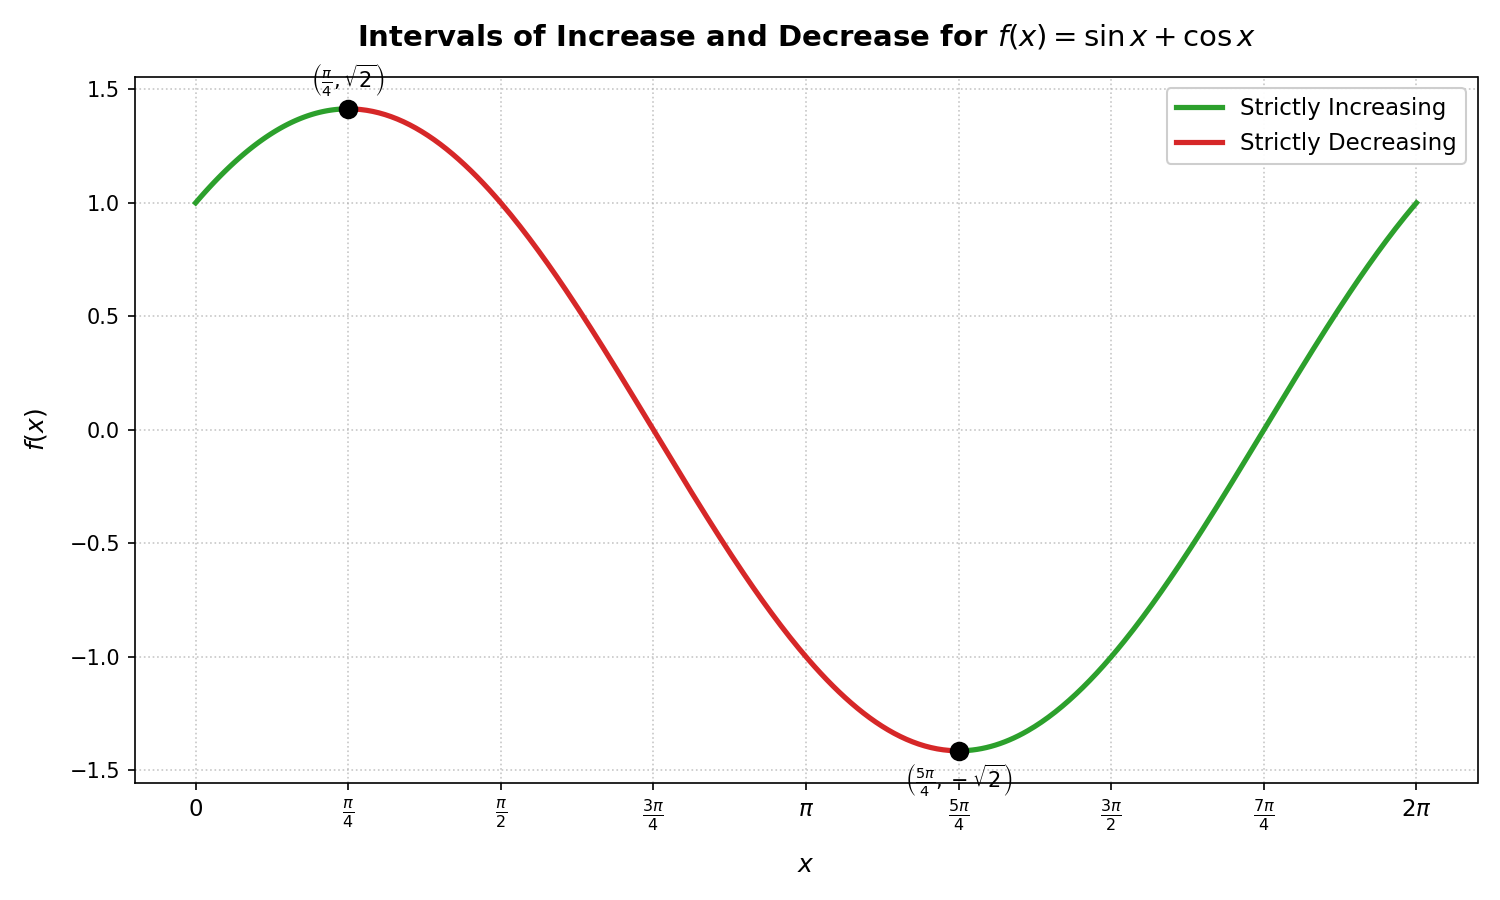
\includegraphics[width=0.6\textwidth]{figs/q11}
  	\caption{Function Representation}
  	\label{Function}
  \end{figure}
  \begin{lstlisting}
  	/codes/q11.py
  \end{lstlisting}
  %=====================Q13================
  \item If $\sin y = x \sin\brak{a + y}$, prove that: $$\frac{dy}{dx} = \frac{\sin^2\brak{a + y}}{\sin a}$$
  
  \solution 
  From \eqref{ITF1}
  \begin{align}
  	F\brak{x, y} = \sin y - x \sin\brak{a + y} = 0
  	\label{eq:state_func}
  \end{align}
  From \eqref{ITF2}
  \begin{align}
  	\frac{dy}{dx} = -\frac{\frac{\partial F}{\partial x}}{\frac{\partial F}{\partial y}}
  	\label{eq:implicit_theorem}
  \end{align}
  
  \begin{align}
  	\frac{\partial F}{\partial x} &= \frac{\partial}{\partial x}\brak{\sin y - x \sin\brak{a + y}}
  	\\
  	&= -\sin\brak{a + y}
  	\label{eq:EE26BTECH11202-partial_x}
  \end{align}
  From \eqref{eq:cosdif}
  \begin{align}
  	\frac{\partial F}{\partial y} &= \frac{\partial}{\partial y}\brak{\sin y - x \sin\brak{a + y}}
  	\\
  	&= \cos y - x \cos\brak{a + y}  \label{eq:EE26BTECH11202-partial_y}
    \end{align}
    As
    \begin{align}
    	x = \frac{\sin y}{\sin\brak{a + y}}
    	\label{eq:EE26BTECH11202-x_expr}
    \end{align}
     Substituting \eqref{eq:EE26BTECH11202-x_expr} into \eqref{eq:EE26BTECH11202-partial_y}:
     \begin{align}
     	\frac{\partial F}{\partial y} &= \cos y - \brak{\frac{\sin y}{\sin\brak{a + y}}} \cos\brak{a + y}
     	\\
     	&= \frac{\sin\brak{a + y}\cos y - \cos\brak{a + y}\sin y}{\sin\brak{a + y}}
     \end{align}
     From \eqref{sinsub}
     \begin{align}
     	\sin\brak{a + y}\cos y - \cos\brak{a + y}\sin y = \sin\brak{a + y - y} = \sin a
     \end{align}
     \begin{align}
     	\frac{\partial F}{\partial y} = \frac{\sin a}{\sin\brak{a + y}}
     	\label{eq:EE26BTECH11202-partial_y_simplified}
     \end{align}
     Substituting \eqref{eq:EE26BTECH11202-partial_x} and \eqref{eq:EE26BTECH11202-partial_y_simplified} into \eqref{eq:implicit_theorem}:
     \begin{align}
     	\frac{dy}{dx} &= -\frac{-\sin\brak{a + y}}{\frac{\sin a}{\sin\brak{a + y}}}
     	\\
     	&= \frac{\sin^2\brak{a + y}}{\sin a}
     \end{align}
    
  %===================Q14=====================
  \item If $\brak{\cos x}^y = \brak{\sin y}^x$, find $\frac{dy}{dx}$.
  \solution
  \begin{align}
  	\ln\brak{\brak{\cos x}^y} &= \ln\brak{\brak{\sin y}^x}
  	\\
  	\implies y \ln\brak{\cos x} &= x \ln\brak{\sin y}
  \end{align}
  From \eqref{ITF1}
  \begin{align}
  	F\brak{x, y} = y \ln\brak{\cos x} - x \ln\brak{\sin y} = 0
  	\label{functional}
  \end{align}
 
  \begin{align}
  \frac{\partial F}{\partial x} &= \frac{\partial}{\partial x}\brak{y \ln\brak{\cos x} - x \ln\brak{\sin y}}
  \\
  &= y \cdot \frac{1}{\cos x} \cdot \brak{-\sin x} - \ln\brak{\sin y} \cdot 1
  \\
  &= -y \tan x - \ln\brak{\sin y}
  \label{partial_x_val}
  \end{align}
  \begin{align}
  	\frac{\partial F}{\partial y} &= \frac{\partial}{\partial y}\brak{y \ln\brak{\cos x} - x \ln\brak{\sin y}}
  	\\
  	&= \ln\brak{\cos x} \cdot 1 - x \cdot \frac{1}{\sin y} \cdot \cos y
  	\\
  	&= \ln\brak{\cos x} - x \cot y
  	\label{partial_y_val}
  \end{align}
   From \eqref{ITF2}
   \begin{align}
   	\frac{dy}{dx} &= -\frac{-y \tan x - \ln\brak{\sin y}}{\ln\brak{\cos x} - x \cot y}
   	\\
   	&= \frac{y \tan x + \ln\brak{\sin y}}{\ln\brak{\cos x} - x \cot y}
   \end{align}
  %==================Q15=====================
  \item 
    Evaluate:
    $$\int x \sin^{-1} x \, dx$$
    \solution
    Let $x = \sin t \implies dx = \cos t \, dt$ and $t = \sin^{-1} x$:
    \begin{align}
    	I\brak{t} &= \int \brak{\sin t} \cdot t \cdot \brak{\cos t \, dt}
    	\\
    	&= \int t \brak{\sin t \cos t} dt
    	\\
    	&= \frac{1}{2} \int t \sin\brak{2t} \, dt
    	\label{eq:EE26BTECH11202-time_integral}
    \end{align}
    Let $g\brak{t} = t \sin\brak{2t}$. Applying \eqref{laplace_sin}, \eqref{laplace_freq_diff}:
    \begin{align}
    	\brak{\sin\brak{2t}} \system{L} \frac{2}{s^2 + 4}
    	\\
    	\implies G\brak{s} = \brak{t \sin\brak{2t}} \system{L}  -\frac{d}{ds} \brak{\frac{2}{s^2 + 4}}
    	\\
    	&= -\brak{\frac{-2 \cdot 2s}{\brak{s^2 + 4}^2}} = \frac{4s}{\brak{s^2 + 4}^2}
    	\label{eq:EE26BTECH11202-G_s}
    \end{align}
    Applying the integration property \eqref{laplace_integration} to $G\brak{s}$:
    \begin{align}
    	H\brak{s} = \brak{\int_0^t \tau \sin\brak{2\tau} d\tau} \system{L} \frac{G\brak{s}}{s}
    	\\
    	&= \frac{1}{s} \cdot \frac{4s}{\brak{s^2 + 4}^2} = \frac{4}{\brak{s^2 + 4}^2}
    	\label{eq:EE26BTECH11202-H_s}
    \end{align}
    Using the transform pair \eqref{laplace_inv_pair} 
    \begin{align}
    	\mathcal{L}^{-1}\brak{\frac{2\brak{2}^3}{\brak{s^2 + 2^2}^2}} = \mathcal{L}^{-1}\brak{\frac{16}{\brak{s^2 + 4}^2}} = \sin\brak{2t} - 2t \cos\brak{2t}
    \end{align}
    Dividing by $4$ yields the inverse transform of $H\brak{s}$ from \eqref{eq:EE26BTECH11202-H_s}:
    \begin{align}
    	\int_0^t \tau \sin\brak{2\tau} d\tau = \mathcal{L}^{-1}\brak{\frac{4}{\brak{s^2 + 4}^2}} = \frac{\sin\brak{2t} - 2t \cos\brak{2t}}{4}
    \end{align}
    	From \eqref{euler_met}
    \begin{figure}[htbp] % [htbp] specifies preferred placement (here, top, bottom, page)
    	\centering
    	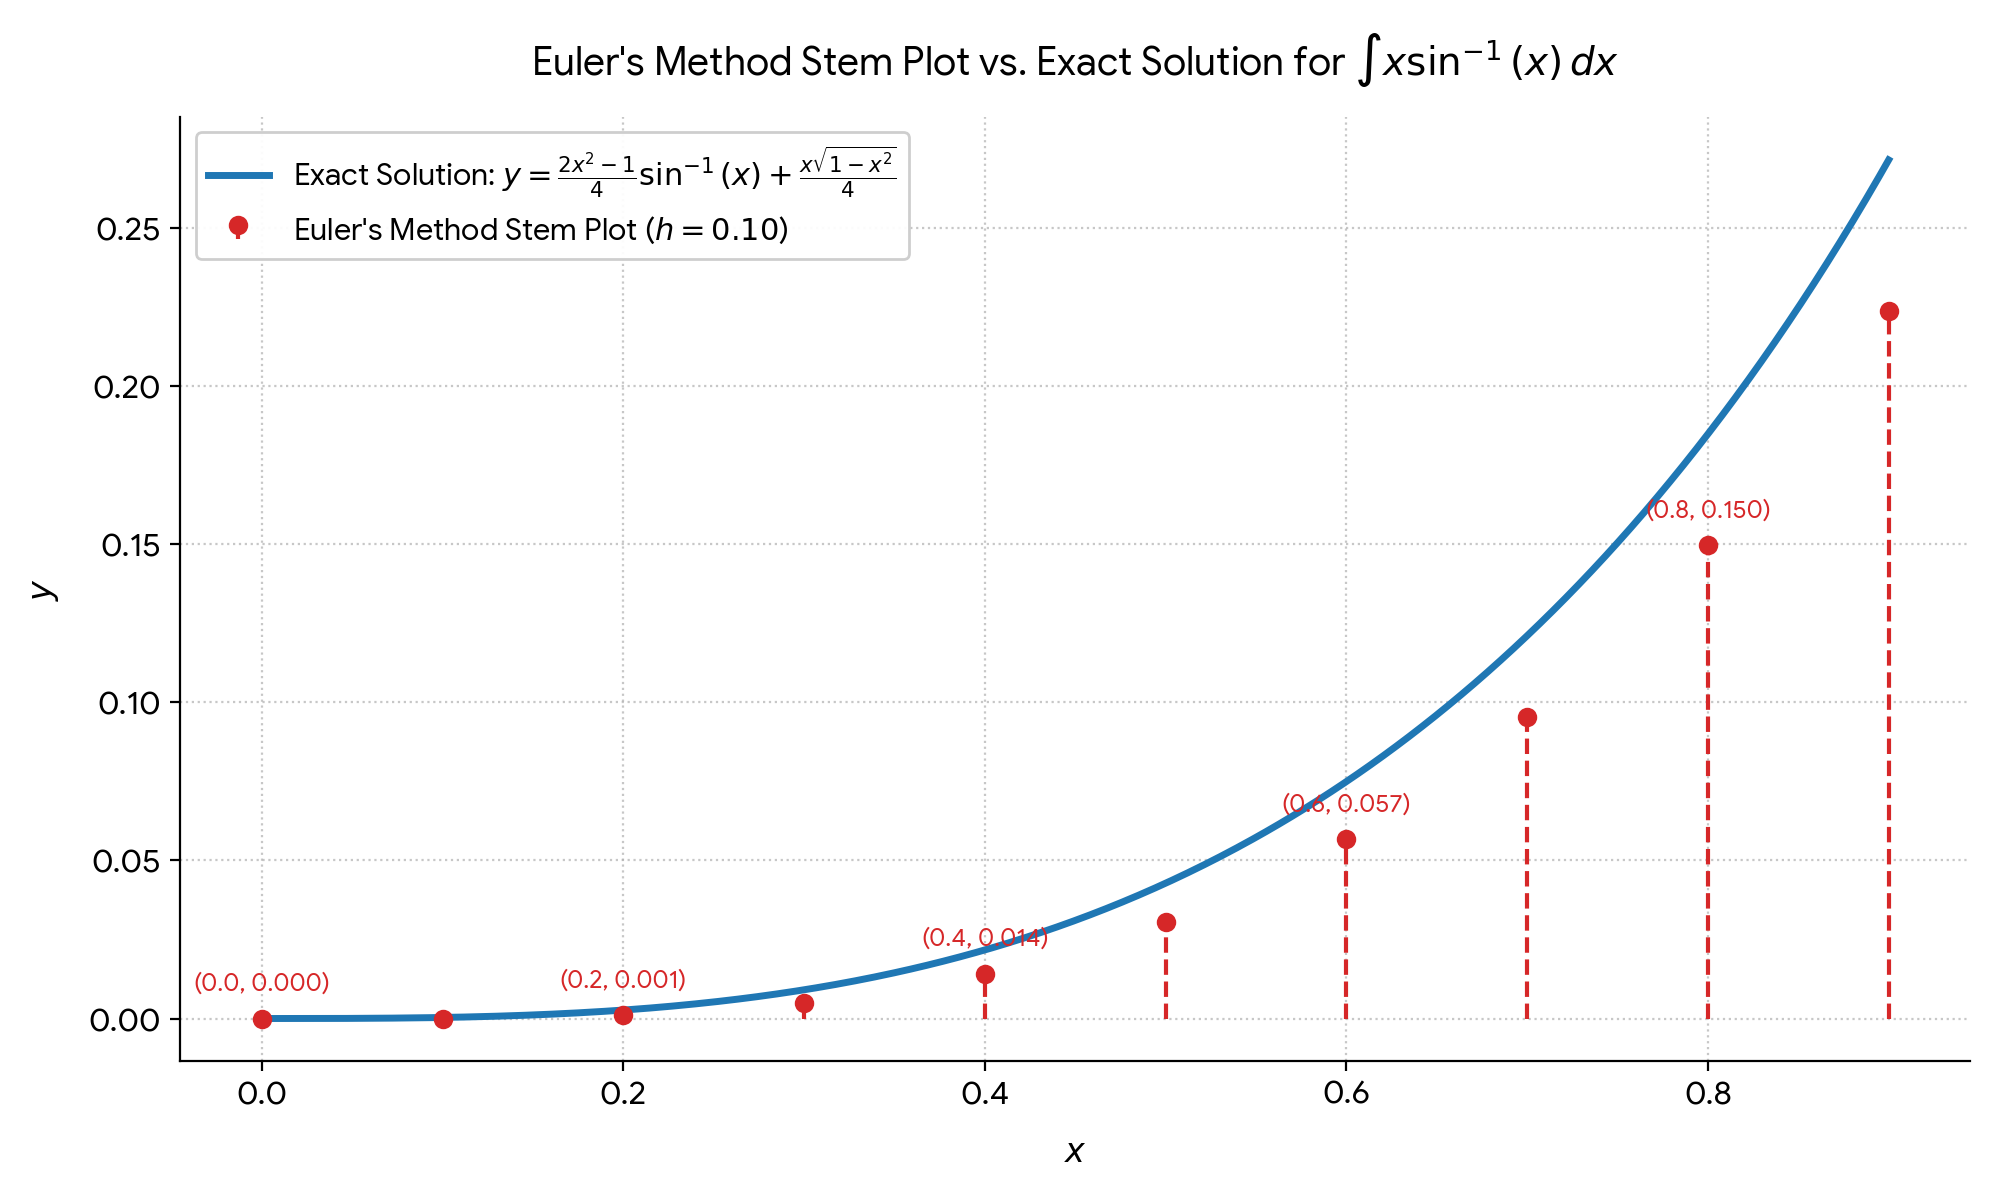
\includegraphics[width=0.6\textwidth]{figs/q14}
    	\caption{Euler method vs Exact solution}
    	\label{euler_fig3}
    \end{figure} \newpage
    \begin{lstlisting}
    	/codes/q14.py
    \end{lstlisting}
  %======================Q16=======
  \item   Prove that:
  $$\cot^{-1}\brak{ \frac{\sqrt{1 + \sin x} + \sqrt{1 - \sin x}}{\sqrt{1 + \sin x} - \sqrt{1 - \sin x}} } = \frac{x}{2}, \quad x \in 0, \brak{\frac{\pi}{4}})$$
  \solution
  
  \begin{align}
  	\frac{x}{2} \in \brak{0, \frac{\pi}{8}}
  \end{align}
  For any angle in the first octant $\brak{0, \frac{\pi}{8}}$:
  \begin{align}
  	\cos\frac{x}{2} > \sin\frac{x}{2} > 0 \implies \cos\frac{x}{2} - \sin\frac{x}{2} > 0
  \end{align}
  Extracting positive real roots for \eqref{eq:EE26BTECH11202-plus_sin_decomp} and \eqref{eq:EE26BTECH11202-minus_sin_decomp}:
  \begin{align}
  	\sqrt{1 + \sin x} &= \mydet{\cos\frac{x}{2} + \sin\frac{x}{2}} = \cos\frac{x}{2} + \sin\frac{x}{2}
  	\label{eq:EE26BTECH11202-radical_plus}
  	\\
  	\sqrt{1 - \sin x} &= \mydet{\cos\frac{x}{2} - \sin\frac{x}{2}} = \cos\frac{x}{2} - \sin\frac{x}{2}
  	\label{eq:EE26BTECH11202-radical_minus}
  \end{align}
  Substituting \eqref{eq:EE26BTECH11202-radical_plus} and \eqref{eq:EE26BTECH11202-radical_minus} into the numeratorand denominator
  
 
  \begin{align}
  	N &= \sqrt{1 + \sin x} + \sqrt{1 - \sin x}
  	\\
  	&= \brak{\cos\frac{x}{2} + \sin\frac{x}{2}} + \brak{\cos\frac{x}{2} - \sin\frac{x}{2}}
  	\\
  	&= 2\cos\frac{x}{2}
  	\label{eq:EE26BTECH11202-num_signal}
  \end{align}
  \begin{align}
  	D &= \sqrt{1 + \sin x} - \sqrt{1 - \sin x}
  	\\
  	&= \brak{\cos\frac{x}{2} + \sin\frac{x}{2}} - \brak{\cos\frac{x}{2} - \sin\frac{x}{2}}
  	\\
  	&= 2\sin\frac{x}{2}
  	\label{den}
  \end{align}
  \begin{align}
  	\frac{N}{D} = \frac{2\cos\frac{x}{2}}{2\sin\frac{x}{2}} = \cot\frac{x}{2}
  \end{align}
  Substituting LHS
  \begin{align}
  	\text{LHS} = \cot^{-1}\brak{\cot\frac{x}{2}}
  \end{align}
  Since $\frac{x}{2} \in \brak{(0, \frac{\pi}{8}}) \subset \brak{0, \pi}$, which lies strictly within the principal branch of $\cot^{-1}\brak{\theta}$, we obtain:
  \begin{align}
  	\cot^{-1}\brak{\cot\frac{x}{2}} = \frac{x}{2} = \text{RHS}
  \end{align}
  
  
  
  
  %=====================Q17========
  \item Solve for $x$:
  $$2 \tan^{-1}\brak{\cos x} = \tan^{-1}2 \brak{\csc x}$$
  \solution
  From \eqref{eq:EE26BTECH11202-double_angle_identity}
  \begin{align}
  	2\tan^{-1}\brak{\cos x} = \tan^{-1}\brak{\frac{2\cos x}{1 - \cos^2 x}}
  \end{align}
  From \eqref{eq:pythogorus}
  \begin{align}
  	2\tan^{-1}\brak{\cos x} = \tan^{-1}\brak{\frac{2\cos x}{\sin^2 x}}
  	\label{eq:EE26BTECH11202-lhs_simplified}
  \end{align}
  Now 
  \begin{align}
  	\tan^{-1}\brak{\frac{2\cos x}{\sin^2 x}} = \tan^{-1}\brak{2\csc x}
  \end{align}
  Taking the tangent of both sides:
  \begin{align}
  	\frac{2\cos x}{\sin^2 x} = 2\csc x = \frac{2}{\sin x}
  	\label{eq:EE26BTECH11202-equated_terms}
  \end{align}
  \begin{align}
  	\frac{2\cos x}{\sin x} &= 2
  	\\
  	\implies \cot x &= 1
  \end{align}
  Taking the inverse cotangent within the principal branch:
  \begin{align}
  	x = \frac{\pi}{4}
  \end{align}
  
  The general solution for $x$ ,
  \begin{align}
  	x = n\pi + \frac{\pi}{4}, \quad n \in \mathbb{Z}
  \end{align}
  %====================Q18============
  \item Find the equation of the tangent to the curve $y = \sqrt{3x - 2}$ which is parallel to the line $4x - 2y + 5 = 0$. \\
  \solution
  \begin{align}
  	4x - 2y + 5 = 0
  \end{align}
  Expressing in  slope-intercept form $y = m_L x + c$:
  \begin{align}
  	2y = 4x + 5 \implies y = 2x + \frac{5}{2}
  \end{align}
  Slope of the parallel line is:
  \begin{align}
  	m = m_L = 2
  	\label{eq:EE26BTECH11202-line_slope}
  \end{align}
  \begin{align}
  	y = \sqrt{3x - 2} = \brak{3x - 2}^{1/2}, \quad \text{for } x > \frac{2}{3}
  \end{align}
   The dynamic slope is $\frac{dy}{dx}$:
  \begin{align}
  	\frac{dy}{dx} = \frac{1}{2\sqrt{3x - 2}} \cdot \frac{d}{dx}\brak{3x - 2} = \frac{3}{2\sqrt{3x - 2}}
  	\label{eq:EE26BTECH11202-curve_derivative}
  \end{align}
  Since they are parallel,slopes are equal
  \begin{align}
  	\frac{3}{2\sqrt{3x_0 - 2}} = 2
  \end{align}
  \begin{align}
  	4\sqrt{3x_0 - 2} = 3 \implies \sqrt{3x_0 - 2} = \frac{3}{4}
  \end{align}
  \begin{align}
  	3x_0 - 2 = \frac{9}{16} \implies 3x_0 = 2 + \frac{9}{16} = \frac{41}{16} \implies x_0 = \frac{41}{48}
  \end{align}
  Substituting $x_0 = \frac{41}{48}$ to find $y_0$:
  \begin{align}
  	y_0 = \sqrt{3\brak{\frac{41}{48}} - 2} = \sqrt{\frac{41}{16} - 2} = \sqrt{\frac{9}{16}} = \frac{3}{4}
  \end{align}
  Line Equation:
 \begin{align}
 	y - \frac{3}{4} = 2\brak{x - \frac{41}{48}}
 \end{align}
 
 \begin{align}
 	y - \frac{3}{4} = 2x - \frac{41}{24}
 \end{align}
 \begin{align}
 	48x - 24y - 23 = 0
 \end{align}
 \begin{figure}[htbp] % [htbp] specifies preferred placement (here, top, bottom, page)
 	\centering
 	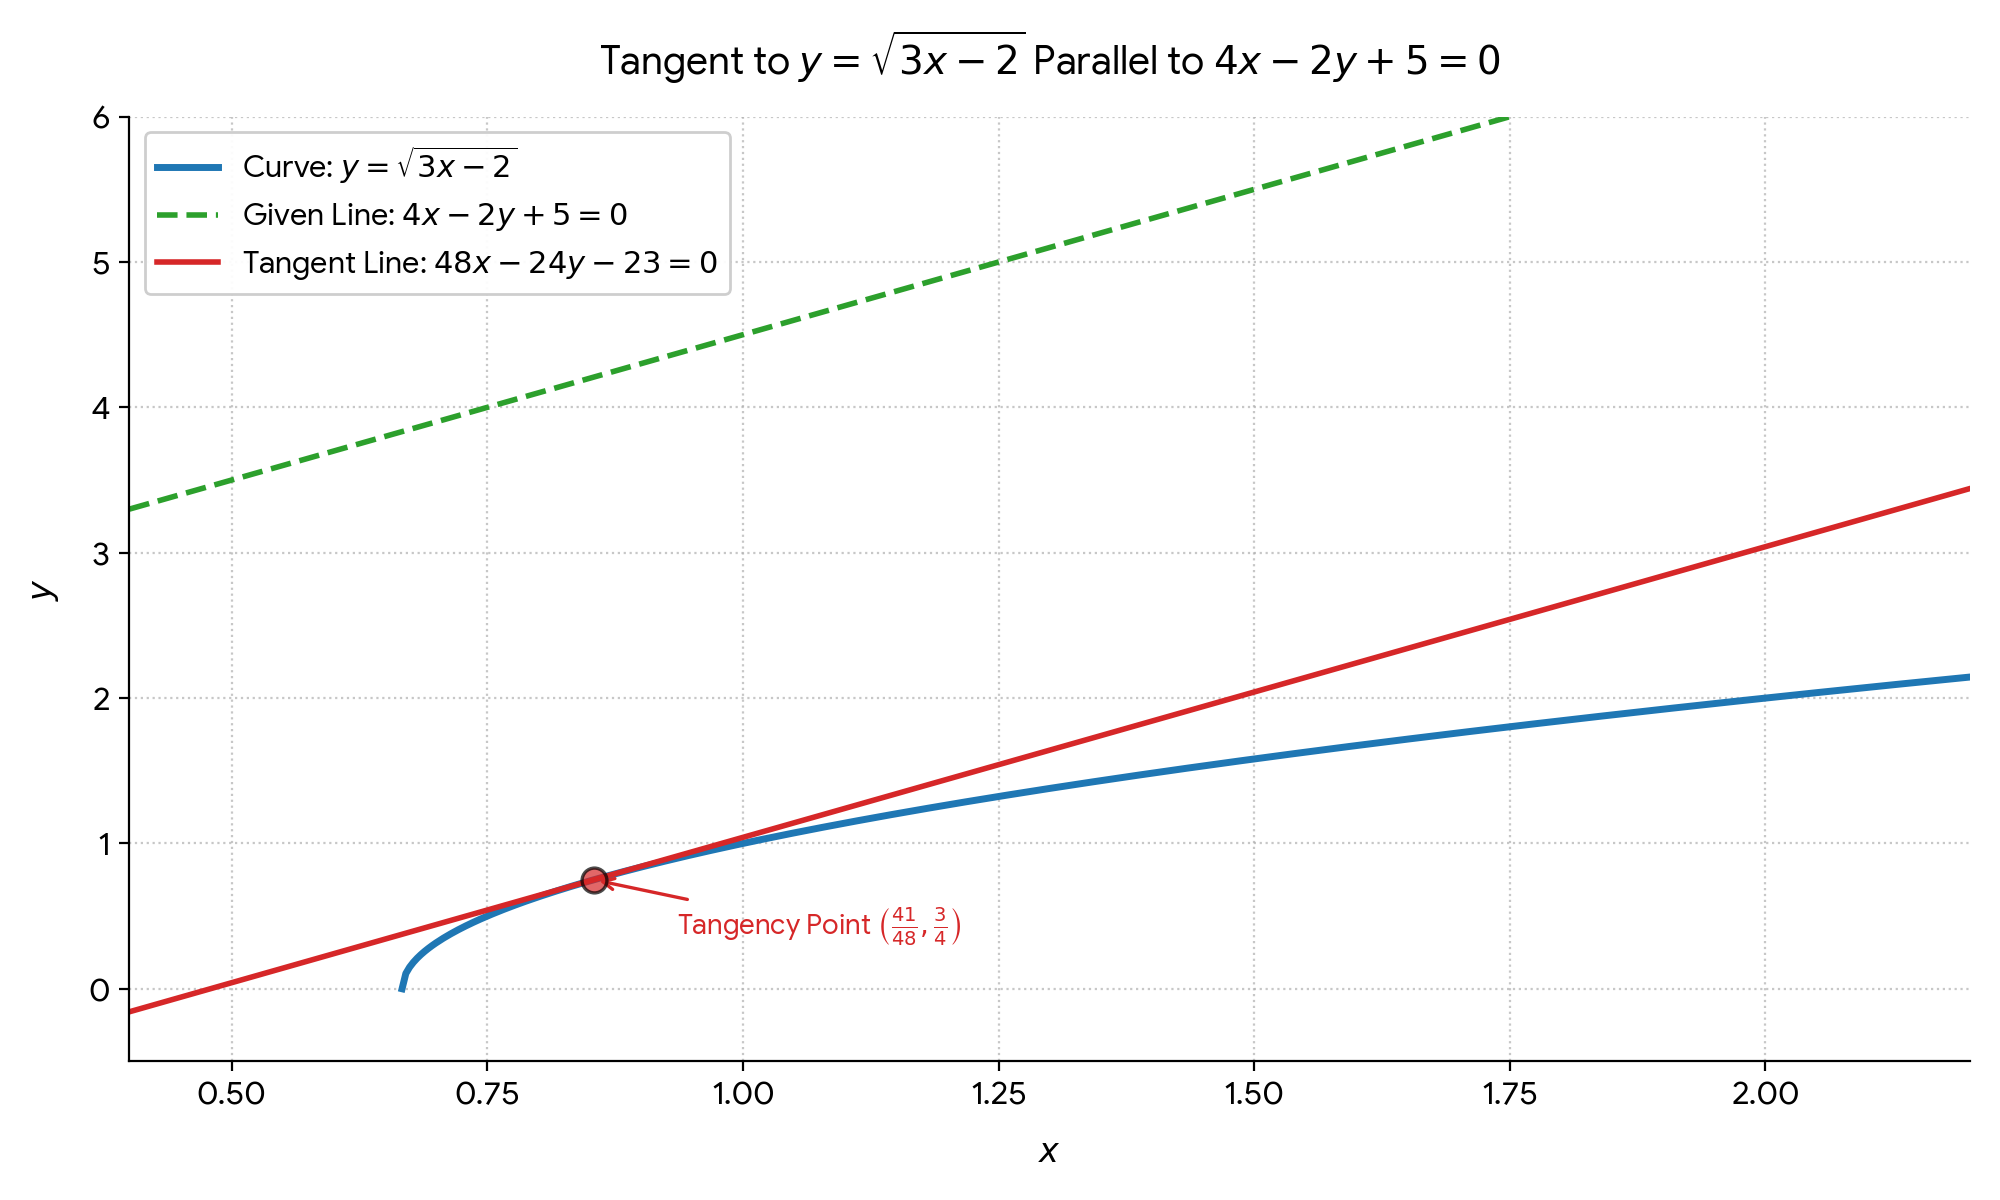
\includegraphics[width=0.6\textwidth]{figs/q17}
 	\caption{Graph}
 	\label{graph_rep}
 \end{figure} \newpage
 \begin{lstlisting}
 	/codes/q17.py
 \end{lstlisting}
 
  %===================Q19================
  \item On a multiple choice examination with three possible answers (out of which only one is correct) for each of the five questions, what is the probability that a candidate would get four or more correct answers just by guessing?\\
  \solution
  Let the discrete random variable $X$ represent the number of correct answers obtained purely by guessing\\
  From \eqref{eq:EE26BTECH11202-pmf}
 
  The event of getting four or more correct answers is $X \ge 4$:
  \begin{align}
  	P\brak{X \ge 4} = P\brak{X = 4} + P\brak{X = 5}
  	\label{eq:EE26BTECH11202-cumulative}
  \end{align}
  \begin{align}
  	P\brak{X = 4} &= \binom{5}{4} \brak{\frac{1}{3}}^4 \brak{\frac{2}{3}}^{5 - 4}
  	\\
  	&= 5 \cdot \frac{1}{81} \cdot \frac{2}{3}
  	\\
  	&= \frac{10}{243}
  	\label{eq:EE26BTECH11202-p4}
  \end{align}
  \begin{align}
  	P\brak{X = 5} &= \binom{5}{5} \brak{\frac{1}{3}}^5 \brak{\frac{2}{3}}^{5 - 5}
  	\\
  	&= 1 \cdot \frac{1}{243} \cdot 1
  	\\
  	&= \frac{1}{243}
  	\label{eq:EE26BTECH11202-p5}
  \end{align}
  \begin{align}
  	P\brak{X \ge 4} &= \frac{10}{243} + \frac{1}{243}
  	\\
  	&= \frac{11}{243}
  \end{align}
  \begin{lstlisting}
  	\codes\q18.py
  	\end{lstlisting}
  %====================Q20===================
 \item Using properties of determinants, prove the following:
  \begin{align*}
  \mydet{1 & 1+p & 1+p+q \\
         2 & 3+2p & 1+3p+2q \\
         3 & 6+3p & 1+6p+3q \\}=1
         \end{align*}
         \solution
         \begin{align}
         	\Delta = \mydet{1 & 1+p & 1+p+q \\
         		2 & 3+2p & 1+3p+2q \\
         		3 & 6+3p & 1+6p+3q} \xrightarrow[R_2 \to R_2 - 2R_1] {R_3 \to R_3 - 3R_1} \mydet{1 & 1+p & 1+p+q \\
         		0 & 1 & -1+p \\
         		0 & 3 & -2+3p} \\ \xrightarrow {R_3 \to R_3 - 3R_2} 
    	\mydet{1 & 1+p & 1+p+q \\
         		0 & 1 & -1+p \\
         		0 & 0 & 1}     
         \end{align}
         The determinant of upper triangular matrix is product of Diagonals
         \begin{align}
         	\Delta &= 1 \cdot \brak{1\cdot 1 - 0\cdot\brak{-1+p}} = 1
         \end{align}
         
         
    %==========================Q21===================
 \item  Solve the following differential equation:
 $$x \frac{dy}{dx} = y - x \tan\brak{\frac{y}{x}}$$
 \solution
 \begin{align}
 	\frac{dy}{dx} = \frac{y}{x} - \tan\brak{\frac{y}{x}}
 	\label{eq:EE26BTECH11202-de_standard}
 \end{align}
 Let 
 \begin{align}
 	v = \frac{y}{x} \implies y = v x
 	\label{eq:EE26BTECH11202-substitution}
 \end{align}
 Differentiating \eqref{eq:EE26BTECH11202-substitution} with respect to $x$ using the product rule:
 \begin{align}
 	\frac{dy}{dx} = v + x \frac{dv}{dx}
 	\label{eq:EE26BTECH11202-diff_sub}
 \end{align}
 \begin{align}
 	v + x \frac{dv}{dx} &= v - \tan\brak{v}
 	\\
 	x \frac{dv}{dx} &= -\tan\brak{v}
 \end{align}
 \begin{align}
 	\frac{dv}{\tan\brak{v}} = -\frac{dx}{x} \implies \cot\brak{v} \, dv = -\frac{dx}{x}
 	\label{eq:EE26BTECH11202-sep_vars}
 \end{align}
 \begin{align}
 	\int \cot\brak{v} \, dv = -\int \frac{dx}{x}
 \end{align}
 \begin{align}
 	\ln  \mydet{\sin\brak{v}} = -\ln \mydet{x} + \ln \mydet{C}
 \end{align}
 \begin{align}
 	\ln \mydet{\sin\brak{v}} = \ln \mydet{\frac{C}{x}} \implies \sin\brak{v} = \frac{C}{x}
 \end{align}
 \begin{align}
 	\sin\brak{\frac{y}{x}} = \frac{C}{x} \implies x \sin\brak{\frac{y}{x}} = C
 	\label{eq:EE26BTECH11202-implicit_general}
 \end{align}
 
 
 	From \eqref{euler_met}
 \begin{figure}[htbp] % [htbp] specifies preferred placement (here, top, bottom, page)
 	\centering
 	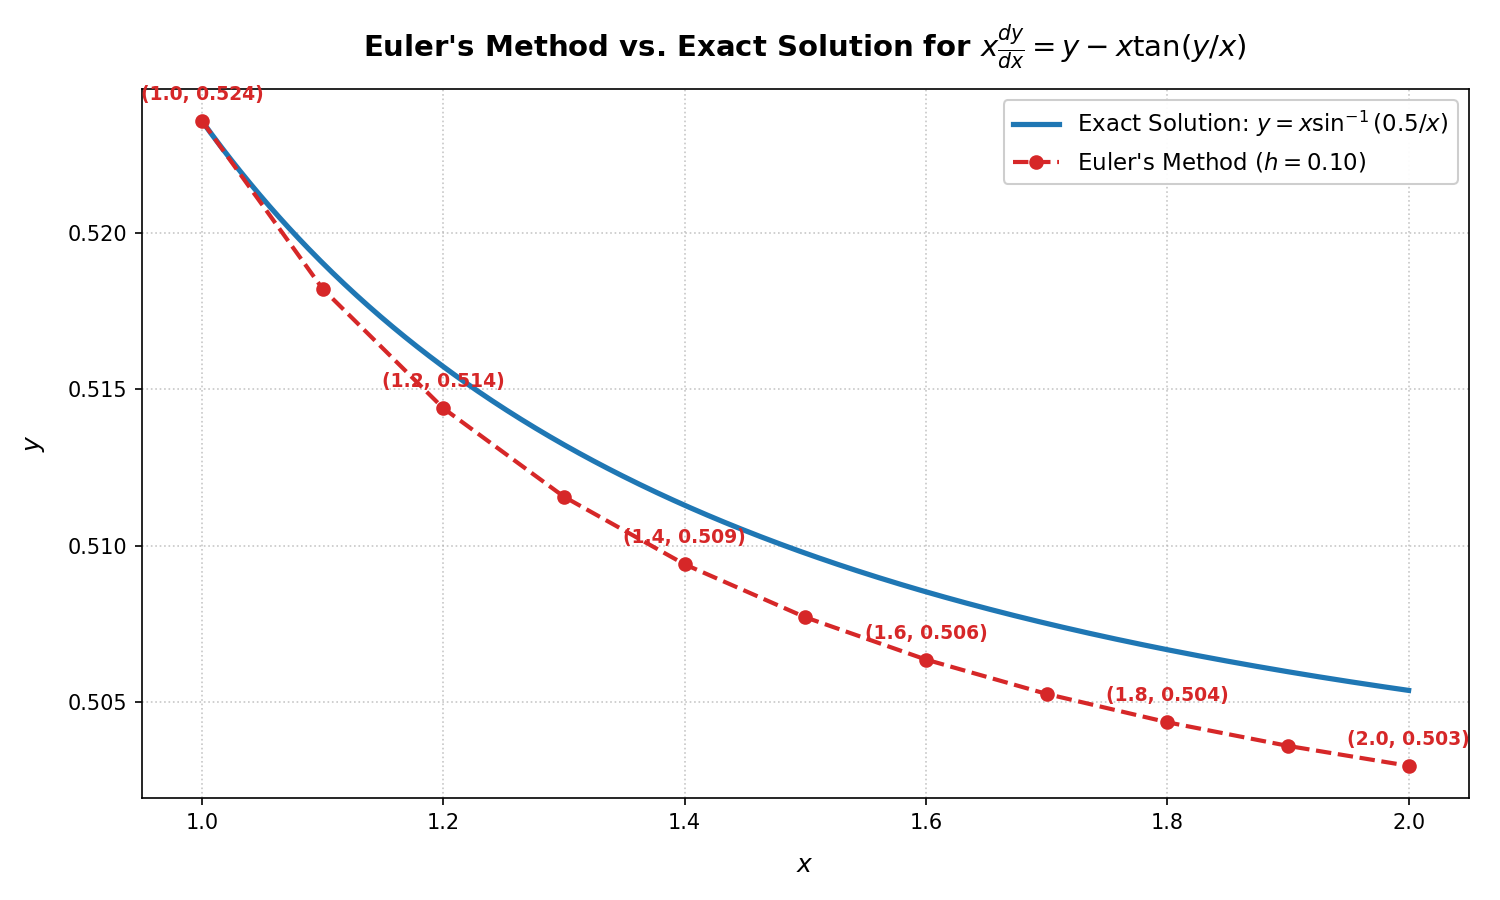
\includegraphics[width=0.6\textwidth]{figs/q20}
 	\caption{Euler's vs Exact }
 	\label{euler_fig4}
 \end{figure} 
 \begin{lstlisting}
 	/codes/q20.py
 \end{lstlisting}
 
 %=====================Q22================
 \item Solve the following differential equation:
 $$\cos^2 x \frac{dy}{dx} + y = \tan x$$
 \solution
 \begin{align}
 	t = \tan x \implies \frac{dt}{dx} = \sec^2 x
 \end{align}
 \begin{align}
 	\frac{dy}{dx} = \frac{dy}{dt} \frac{dt}{dx} = \sec^2 x \frac{dy}{dt}
 	\label{eq:EE26BTECH11202-chain_rule}
 \end{align}
 Substituting \eqref{eq:EE26BTECH11202-chain_rule} into $\cos^2 x \frac{dy}{dx} + y = \tan x$:
 \begin{align}
 	\cos^2 x \brak{\sec^2 x \frac{dy}{dt}} + y = t \implies \frac{dy}{dt} + y = t
 	\label{eq:EE26BTECH11202-lti_system}
 \end{align}
 \begin{align}
 	s Y(s) - y(0^-) + Y(s) = \frac{1}{s^2}
 \end{align}
 Solving for $Y(s)$:
 \begin{align}
 	(s + 1) Y(s) &= \frac{1}{s^2} + y(0^-)
 	\\
 	Y(s) &= \frac{1}{s^2(s + 1)} + \frac{y(0^-)}{s + 1}
 	\label{eq:EE26BTECH11202-laplace_domain}
 \end{align}
 \begin{align}
 	\frac{1}{s^2(s + 1)} = \frac{A}{s} + \frac{B}{s^2} + \frac{C_0}{s + 1}
 \end{align}
 Solving coefficients: $B = 1$, $C_0 = 1$, $A = -1$:
 \begin{align}
 	Y(s) = \frac{1}{s^2} - \frac{1}{s} + \frac{1}{s + 1} + \frac{y(0^-)}{s + 1}
 \end{align}
 \begin{align}
 	y(t) = t - 1 + \brak{1 + y(0^-)} e^{-t} = t - 1 + C e^{-t}
 \end{align}
 Substituting back $t = \tan x$:
 \begin{align}
 	y(x) = \tan x - 1 + C e^{-\tan x}
 \end{align}
 	From \eqref{euler_met}
 \begin{figure}[htbp] % [htbp] specifies preferred placement (here, top, bottom, page)
 	\centering
 	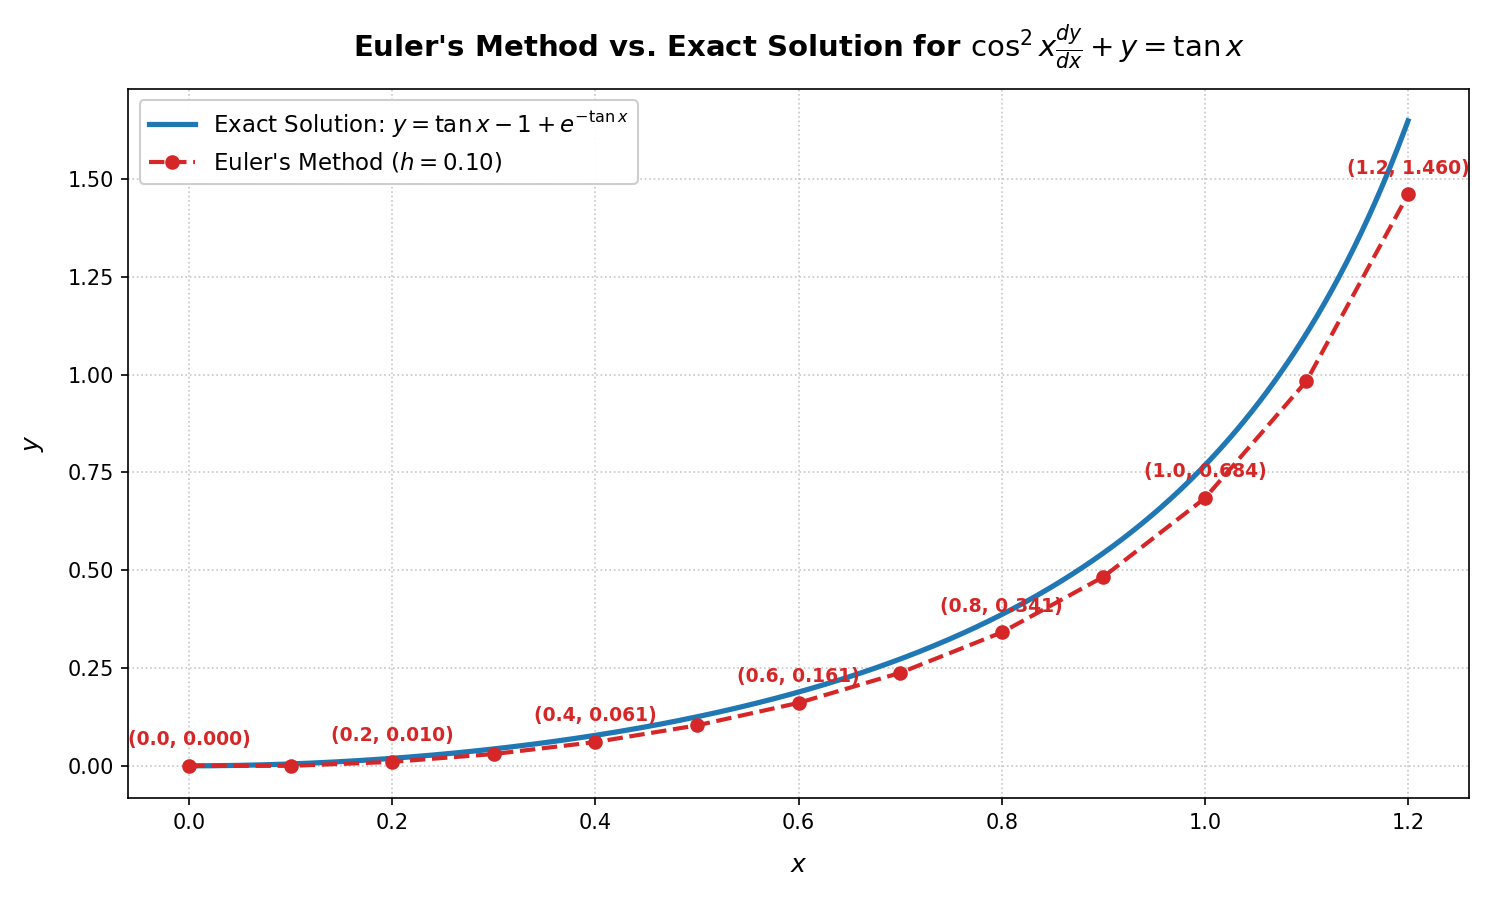
\includegraphics[width=0.6\textwidth]{figs/q21}
 	\caption{Euler's vs Exact }
 	\label{euler_fig5}
 \end{figure} 
 \begin{lstlisting}
 	/codes/q21.py
 \end{lstlisting}
 
 %===============Q23===============
 \item Find a unit vector perpendicular to each of the vectors $\vec{a} + \vec{b}$ and $\vec{a} - \vec{b}$, where $\vec{a} = \vec{e}_1 +\vec{e}_2 + \vec{e}_3$ and ${\vec{b} = \vec{e}_1 + 2\vec{e}_2 + 3\vec{e}_3}$.\\
 \solution
 $\vec{v} = \vec{a} - \vec{b}$
 \begin{align}
 	\vec{v} &= \brak{1 - 1}\vec{e}_1 + \brak{1 - 2}\vec{e}_2 + \brak{1 - 3}\vec{e}_3
 	\\
 	&= 0\vec{e}_1 - \vec{e}_2 - 2\vec{e}_3 = \myvec{0 \\ -1 \\ -2}
 \end{align}
 From \eqref{eq:cross}
 \begin{align}
 	\vec{w} &= \vec{u} \times \vec{v}
 	\\
 	&= \myvec{3\brak{-2} - 4\brak{-1} \\ 4\brak{0} - 2\brak{-2} \\ 2\brak{-1} - 3\brak{0}}
 	\\
 	&= \myvec{-6 + 4 \\ 0 + 4 \\ -2 - 0} = \myvec{-2 \\ 4 \\ -2} 	
 \end{align}
 \begin{align}
 	\norm{\vec{w}} &= \sqrt{\brak{-2}^2 + 4^2 + \brak{-2}^2}
 	\\
 	&= \sqrt{4 + 16 + 4} = \sqrt{24} = 2\sqrt{6}
 \end{align}
  \begin{align}
  From \eqref{unit_vector}
  	\\
  	&= \pm \frac{-2\vec{e}_1 + 4\vec{e}_2 - 2\vec{e}_3}{2\sqrt{6}}
  	\\
  	&= \pm \frac{1}{\sqrt{6}}\brak{-\vec{e}_1 + 2\vec{e}_2 - \vec{e}_3}
  \end{align}
 \begin{figure}[htbp] % [htbp] specifies preferred placement (here, top, bottom, page)
 	\centering
 	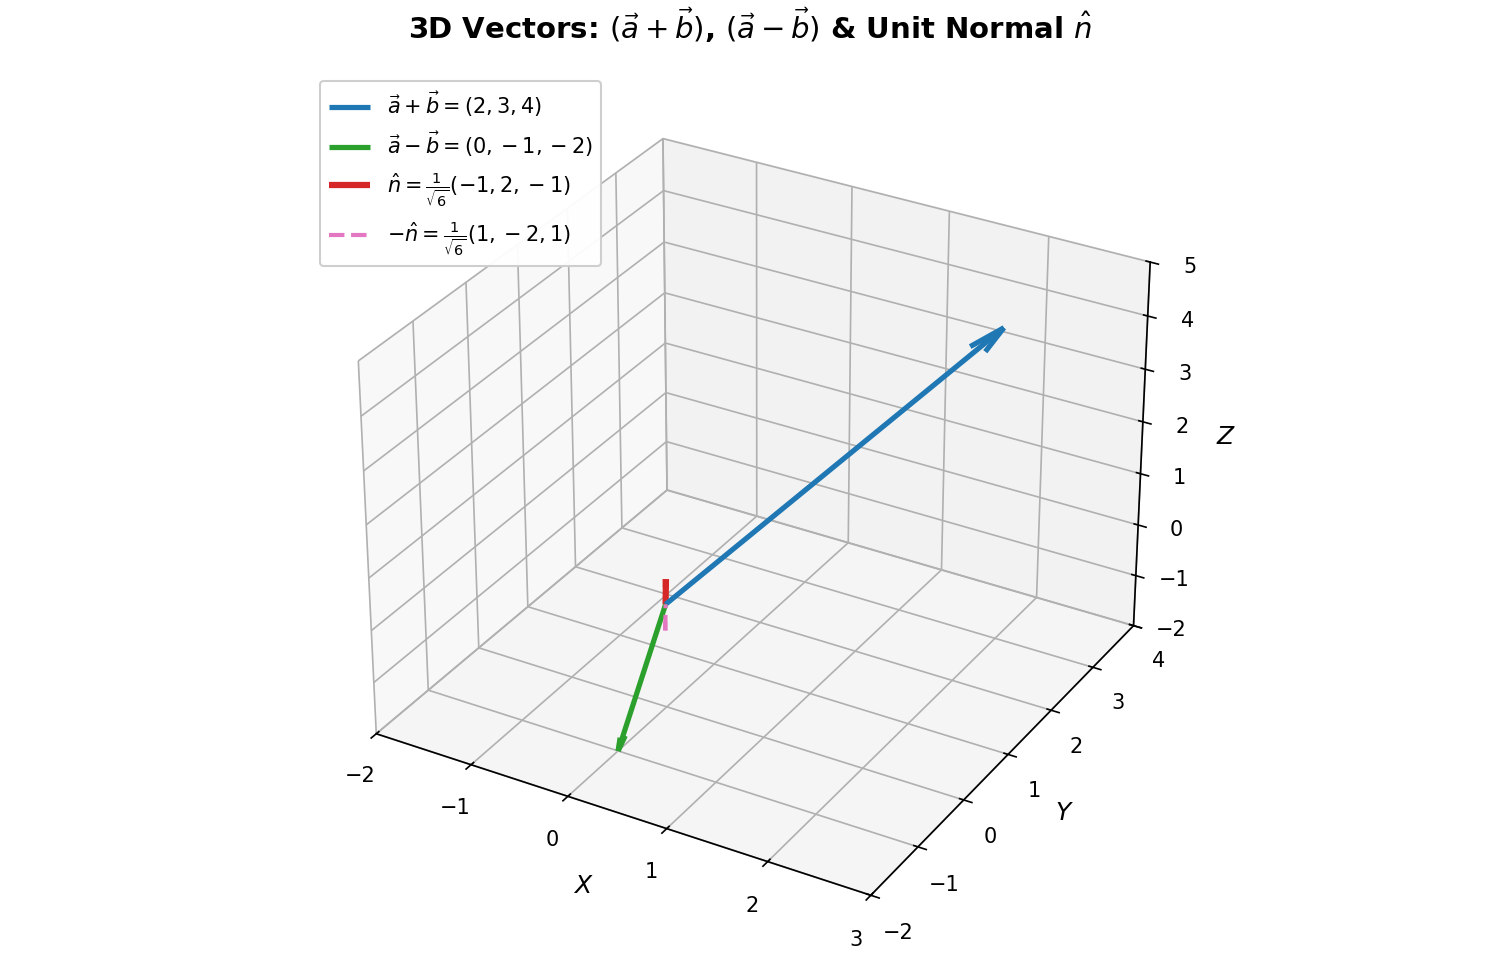
\includegraphics[width=0.6\textwidth]{figs/q22}
 	\caption{Graphical Representation}
 	\label{vec_per}
 \end{figure} 
 \begin{lstlisting}
 	/codes/q22.py
 \end{lstlisting}
 
 %================Q24==================
 \item Find the shortest distance between the lines $\vec{r} = \brak{\vec{e}_1+ 2 \vec{e}_2 +  \vec{e}_3} + \lambda\brak{\vec{e}_1 -  \vec{e}_2 +  \vec{e}_3}$ and $\vec{r} = \brak{2 \vec{e}_1 -  \vec{e}_2-  \vec{e}_3} + \mu\brak{2 \vec{e}_1 +  \vec{e}_2 + 2 \vec{e}_3}$.\\
 \solution
 \begin{align}
 	L_1: \vec{r}_1 &= \vec{a}_1 + \lambda \vec{b}_1
 	\\
 	L_2: \vec{r}_2 &= \vec{a}_2 + \mu \vec{b}_2
 \end{align}
 \begin{align}
 	\vec{a}_1 &= \myvec{1 \\ 2 \\ 1}, \quad \vec{b}_1 = \myvec{1 \\ -1 \\ 1}
 	\\
 	\vec{a}_2 &= \myvec{2 \\ -1 \\ -1}, \quad \vec{b}_2 = \myvec{2 \\ 1 \\ 2}
 \end{align}
 The relative displacement vector $\vec{a}_2 - \vec{a}_1$ connecting the two line reference points is:
 \begin{align}
 	\vec{a}_2 - \vec{a}_1 &= \myvec{2 - 1 \\ -1 - 2 \\ -1 - 1} = \myvec{1 \\ -3 \\ -2}
 	\label{eq:EE26BTECH11202-disp_vec}
 \end{align}
 Normal vector $\vec{n} = \vec{b}_1 \times \vec{b}_2$
 \begin{align}
 	From \eqref{eq:cross} \\
 \vec{n} &= \myvec{\brak{-1}\brak{2} - \brak{1}\brak{1} \\ \brak{1}\brak{2} - \brak{1}\brak{2} \\ \brak{1}\brak{1} - \brak{-1}\brak{2}}
 	\\
 	&= \myvec{-2 - 1 \\ 2 - 2 \\ 1 + 2} = \myvec{-3 \\ 0 \\ 3}
 	\label{eq:EE26BTECH11202-normal_vec}
 \end{align}
 \begin{align}
 	\norm{\vec{n}} &= \sqrt{\brak{-3}^2 + 0^2 + 3^2}
 	\\
 	&= \sqrt{9 + 0 + 9} = \sqrt{18} = 3\sqrt{2}
 	\label{eq:EE26BTECH11202-norm_eval}
 \end{align}
 Evaluating the inner product
 \begin{align}
 	\brak{\vec{a}_2 - \vec{a}_1}^T \vec{n} &= \myvec{1 & -3 & -2} \myvec{-3 \\ 0 \\ 3}
 	\\
 	&= \brak{1}\brak{-3} + \brak{-3}\brak{0} + \brak{-2}\brak{3}
 	\\
 	&= -3 + 0 - 6 = -9
 \end{align}
 From \eqref{shortest_distance}
 \begin{align}
 	d = \frac{|-9|}{3\sqrt{2}} = \frac{9}{3\sqrt{2}} = \frac{3}{\sqrt{2}} = \frac{3\sqrt{2}}{2}
 \end{align}
  \begin{figure}[htbp] % [htbp] specifies preferred placement (here, top, bottom, page)
 	\centering
 	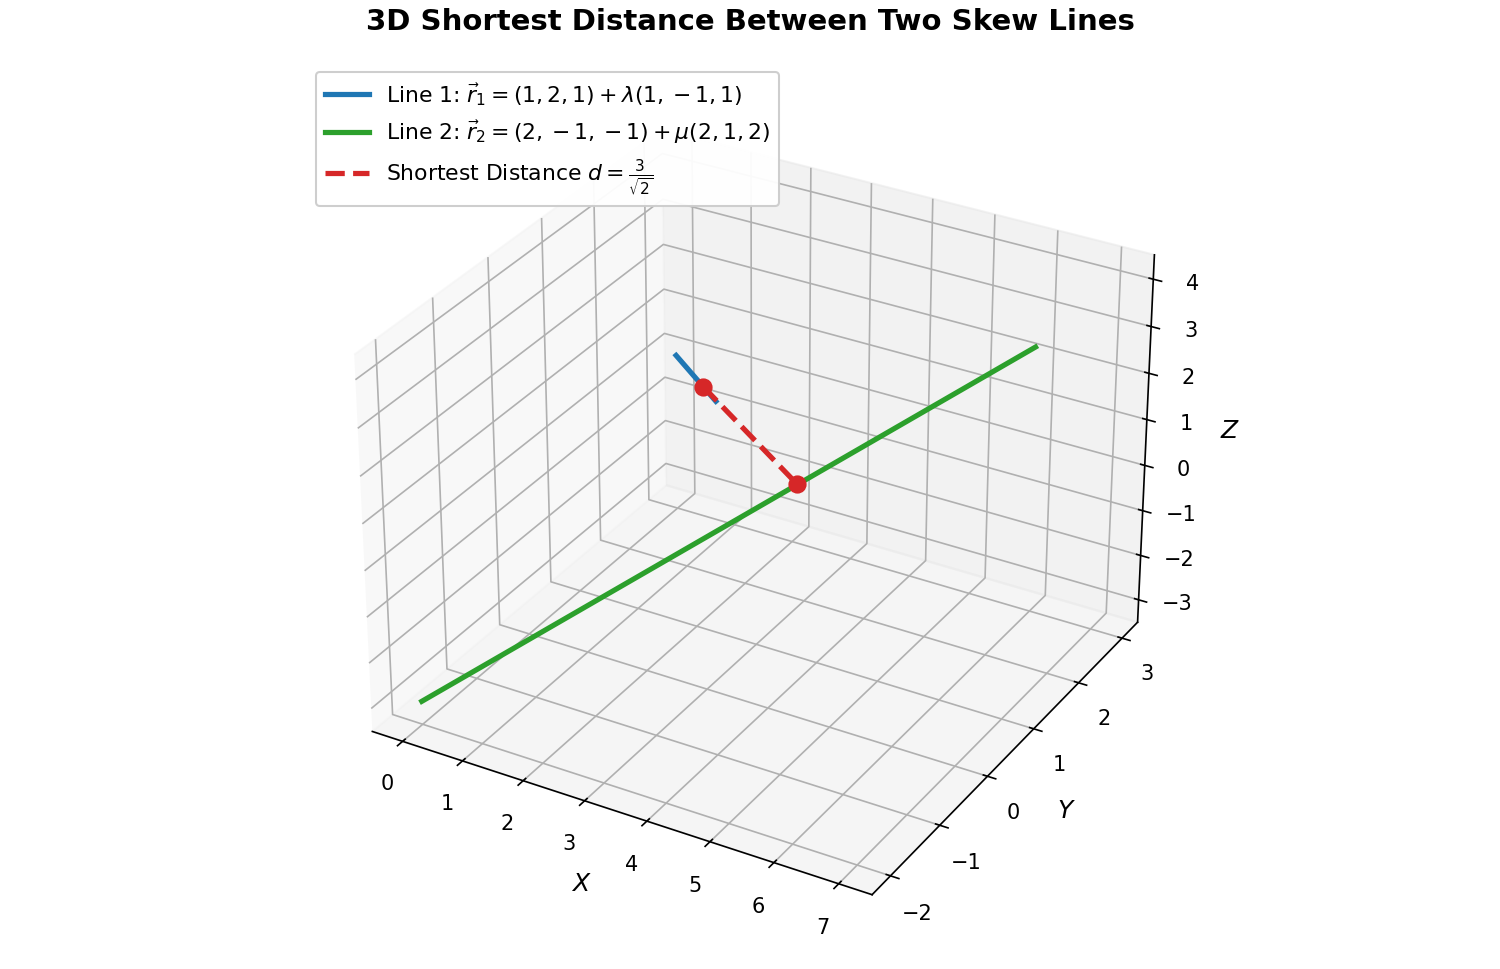
\includegraphics[width=0.6\textwidth]{figs/q23}
 	\caption{Graphical Representation}
 	\label{shor_dis}
 \end{figure} \newpage 
 \begin{lstlisting}
 	/codes/q23.py
 \end{lstlisting}
 
 %====================Q25============
 \item The scalar product of the vector $\vec{e}_1 + \vec{e}_2 + \vec{e}_3$ with the unit vector along the sum of vectors $2\vec{e}_1 + 4\vec{e}_2- 5\vec{e}_3$ and $\lambda \vec{e}_1 + 2\vec{e}_2 + 3\vec{e}_3$ is equal to one. Find the value of $\lambda$.
 \solution
 \begin{align}
 	\vec{x} &= \vec{e}_1 + \vec{e}_2 + \vec{e}_3 = \myvec{1 \\ 1 \\ 1}
 	\\
 	\vec{u} &= 2\vec{e}_1 + 4\vec{e}_2 - 5\vec{e}_3 = \myvec{2 \\ 4 \\ -5}
 	\\
 	\vec{v} &= \lambda \vec{e}_1 + 2\vec{e}_2 + 3\vec{e}_3 = \myvec{\lambda \\ 2 \\ 3}
 \end{align}
 Let: $\vec{w} = \vec{u} + \vec{v}$
 \begin{align}
 \vec{w} &= \myvec{2 + \lambda \\ 4 + 2 \\ -5 + 3} = \myvec{2 + \lambda \\ 6 \\ -2}
 \label{eq:EE26BTECH11202-sum_vector}
 \end{align}
 From \eqref{unit_vector}
\begin{align}
	\vec{x}^T \hat{w} = 1 \implies \frac{\vec{x}^T \vec{w}}{\norm{\vec{w}}} = 1 \implies \vec{x}^T \vec{w} = \norm{\vec{w}}
	\label{eq:EE26BTECH11202-projection_cond}
\end{align}
Evaluating the numerator $\vec{x}^T \vec{w}$ using matrix transposition:
\begin{align}
	\vec{x}^T \vec{w} &= \myvec{1 & 1 & 1} \myvec{2 + \lambda \\ 6 \\ -2}
	\\
	&= \brak{1}\brak{2 + \lambda} + \brak{1}\brak{6} + \brak{1}\brak{-2}
	\\
	&= 2 + \lambda + 6 - 2 = \lambda + 6
	\label{eq:EE26BTECH11202-dot_eval}
\end{align}
\begin{align}
	\lambda + 6 = \sqrt{\lambda^2 + 4\lambda + 44}
\end{align}
\begin{align}
	\brak{\lambda + 6}^2 &= \lambda^2 + 4\lambda + 44
	\\
	\lambda^2 + 12\lambda + 36 &= \lambda^2 + 4\lambda + 44
\end{align}
\begin{align}
	12\lambda - 4\lambda &= 44 - 36
	\\
	8\lambda &= 8 \implies \lambda = 1
\end{align}
 %=================Q26==================
 \item Find the equation of the plane determined by the points $A\brak{3, -1, 2}$, $B\brak{5, 2, 4}$ and $C\brak{-1, -1, 6}$. Also find the distance of the point $P\brak{6, 5, 9}$ from the plane.
 \solution
 Position vector:
 \begin{align}
 	\vec{r}_A = \myvec{3 \\ -1 \\ 2}, \quad \vec{r}_B = \myvec{5 \\ 2 \\ 4}, \quad \vec{r}_C = \myvec{-1 \\ -1 \\ 6}, \quad \vec{r}_P = \myvec{6 \\ 5 \\ 9}
 \end{align}
 Let:
 \begin{align}
 	\vec{u} &= \vec{r}_B - \vec{r}_A = \myvec{5 - 3 \\ 2 - \brak{-1} \\ 4 - 2} = \myvec{2 \\ 3 \\ 2}
 	\label{eq:EE26BTECH11202-u_vec}
 	\\
 	\vec{v} &= \vec{r}_C - \vec{r}_A = \myvec{-1 - 3 \\ -1 - \brak{-1} \\ 6 - 2} = \myvec{-4 \\ 0 \\ 4}
 	\label{eq:EE26BTECH11202-v_vec}
 \end{align}
 Normal vector $\vec{n} = \vec{u} \times \vec{v}$ orthogonal to the plane,
 From \eqref{eq:cross}
 \begin{align}
 	\vec{n} &= \myvec{3\brak{4} - 2\brak{0} \\ 2\brak{-4} - 2\brak{4} \\ 2\brak{0} - 3\brak{-4}} = \myvec{12 \\ -8 - 8 \\ 12} = \myvec{12 \\ -16 \\ 12}
 \end{align}
 Scaling down by the common factor of $4$ yields an equivalent direction normal vector $\vec{n}_0$:
 \begin{align}
 	\vec{n}_0 = \myvec{3 \\ -4 \\ 3}
 	\label{eq:EE26BTECH11202-normal_reduced}
 \end{align}
 From \eqref{eq:plane}
 \begin{align}
 	\vec{r}_A^T \vec{n}_0 = \myvec{3 & -1 & 2} \myvec{3 \\ -4 \\ 3} = \brak{3}\brak{3} + \brak{-1}\brak{-4} + \brak{2}\brak{3} = 9 + 4 + 6 = 19
 \end{align}
 \begin{align}
 	\myvec{x & y & z} \myvec{3 \\ -4 \\ 3} = 19 \implies 3x - 4y + 3z = 19
 \end{align}
 Thus, the equation of the plane in Cartesian form is:
 \begin{align}
 	3x - 4y + 3z - 19 = 0
 \end{align}
 From \eqref{eq:per_dis}
 \begin{align}
 	\vec{r}_P^T \vec{n}_0 = \myvec{6 & 5 & 9} \myvec{3 \\ -4 \\ 3} = \brak{6}\brak{3} + \brak{5}\brak{-4} + \brak{9}\brak{3} = 18 - 20 + 27 = 25
 \end{align}
 \begin{align}
 	\norm{\vec{n}_0} = \sqrt{3^2 + \brak{-4}^2 + 3^2} = \sqrt{9 + 16 + 9} = \sqrt{34}
 \end{align}
 \begin{align}
 	d = \frac{|25 - 19|}{\sqrt{34}} = \frac{6}{\sqrt{34}} = \frac{3\sqrt{34}}{17}
 \end{align}
 \begin{figure}[htbp] % [htbp] specifies preferred placement (here, top, bottom, page)
 	\centering
 	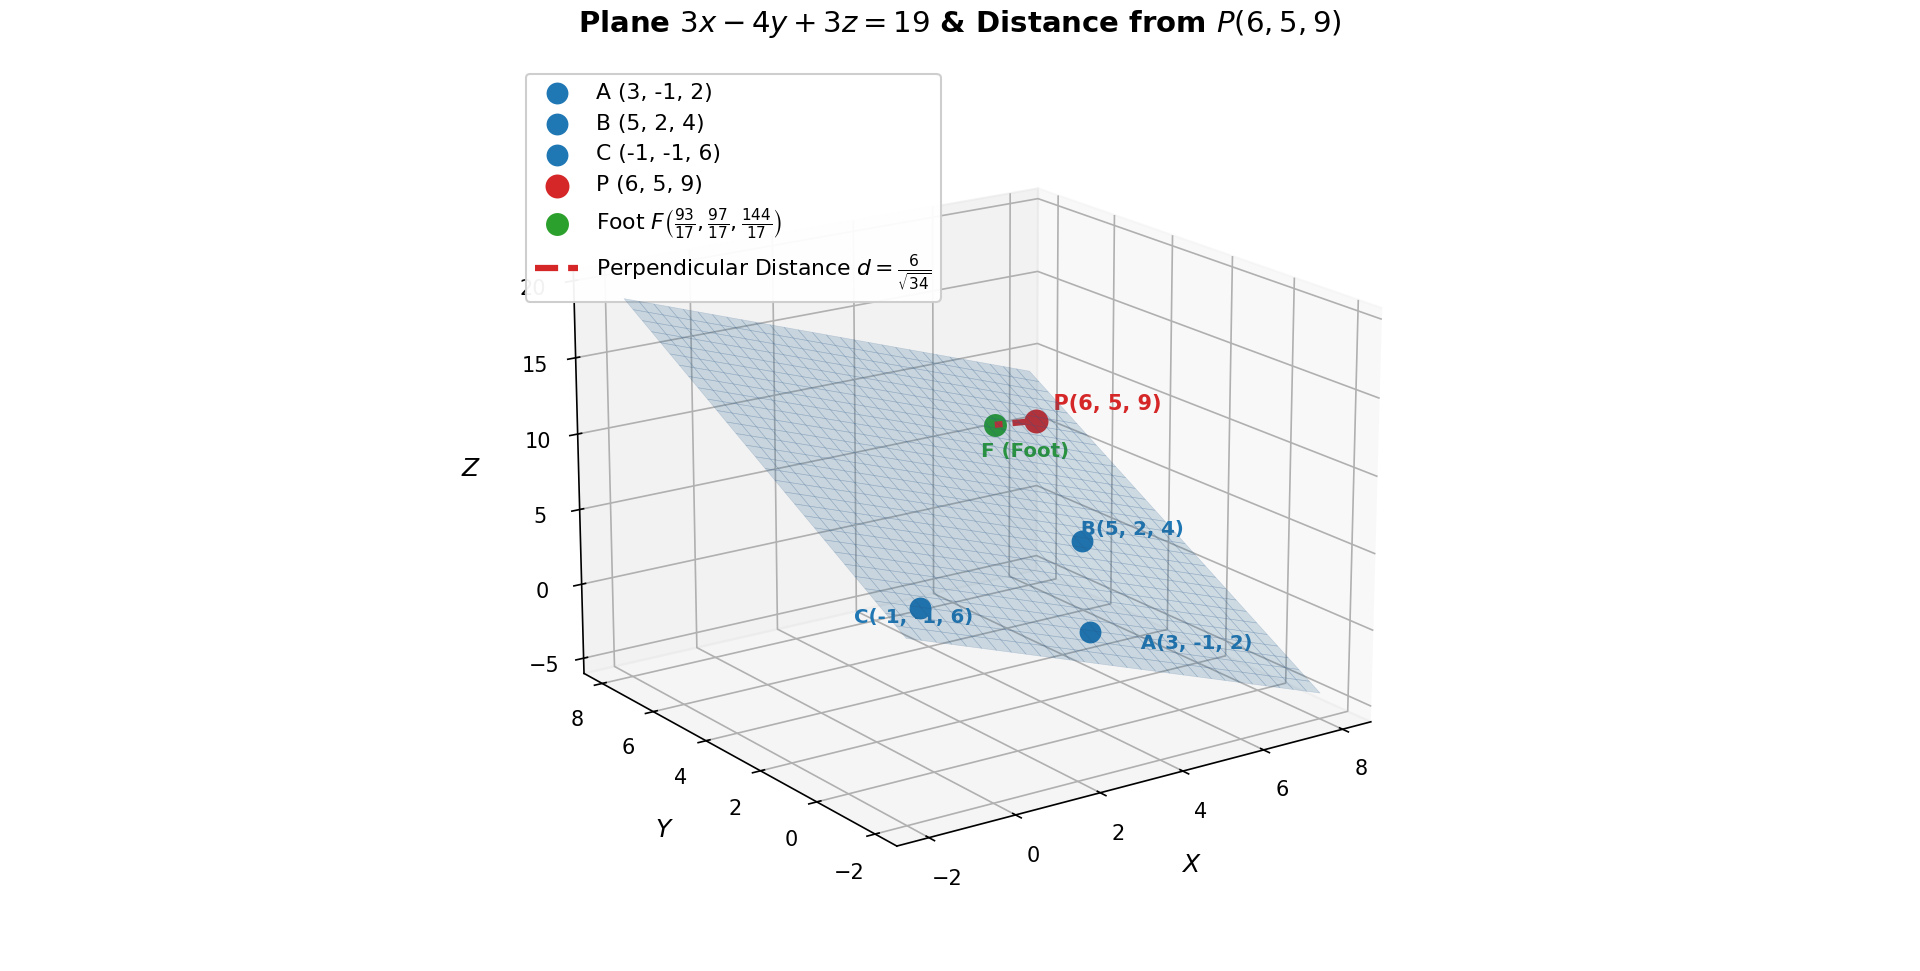
\includegraphics[width=0.6\textwidth]{figs/q25}
 	\caption{Graphical Representation}
 	\label{plane_dis}
 \end{figure}  
 \begin{lstlisting}
 	/codes/q25.py
 \end{lstlisting}
 
 %========Q27====================
 \item Find the area of the region included between the parabola $y^2 = x$ and the line $x + y = 2$.\\
 \solution
 Equating the $x$-coordinates
 \begin{align}
 	y^2 = 2 - y \implies y^2 + y - 2 = 0
 \end{align}
 \begin{align}
 	\brak{y + 2}\brak{y - 1} = 0 \implies y_1 = -2, \quad y_2 = 1
 \end{align}
 Substituting the roots
 \begin{align}
 	 y_1 = -2: & \quad x_1 = \brak{-2}^2 = 4 \implies B\brak{4, -2}
 	\\
 	 y_2 = 1: & \quad x_2 = \brak{1}^2 = 1 \implies A\brak{1, 1}
 \end{align}
 The area is given by:
 \begin{align}
 	\text{Area}\brak{\Omega} &= \int_{y=-2}^{y=1} \brak{x_R\brak{y} - x_L\brak{y}} \, dy
 	\\
 	&= \int_{-2}^{1} \brak{2 - y - y^2} \, dy \\
 	 &= \brak{2y - \frac{y^2}{2} - \frac{y^3}{3}}_{-2}^{1}
 	\\
 	&= \brak{2\brak{1} - \frac{1^2}{2} - \frac{1^3}{3}} - \brak{2\brak{-2} - \frac{\brak{-2}^2}{2} - \frac{\brak{-2}^3}{3}}
 	\\
 	&= \brak{2 - \frac{1}{2} - \frac{1}{3}} - \brak{-4 - 2 + \frac{8}{3}}
 	\\
 	&= \brak{\frac{7}{6}} - \brak{-6 + \frac{8}{3}}
 	\\
 	&= \frac{7}{6} - \brak{-\frac{10}{3}} = \frac{7}{6} + \frac{20}{6} = \frac{27}{6} \\
 	\text{Area}\brak{\Omega} &= \frac{9}{2} \text{ square units}
 \end{align}
 
 	\begin{figure}[htbp] % [htbp] specifies preferred placement (here, top, bottom, page)
 	\centering
 	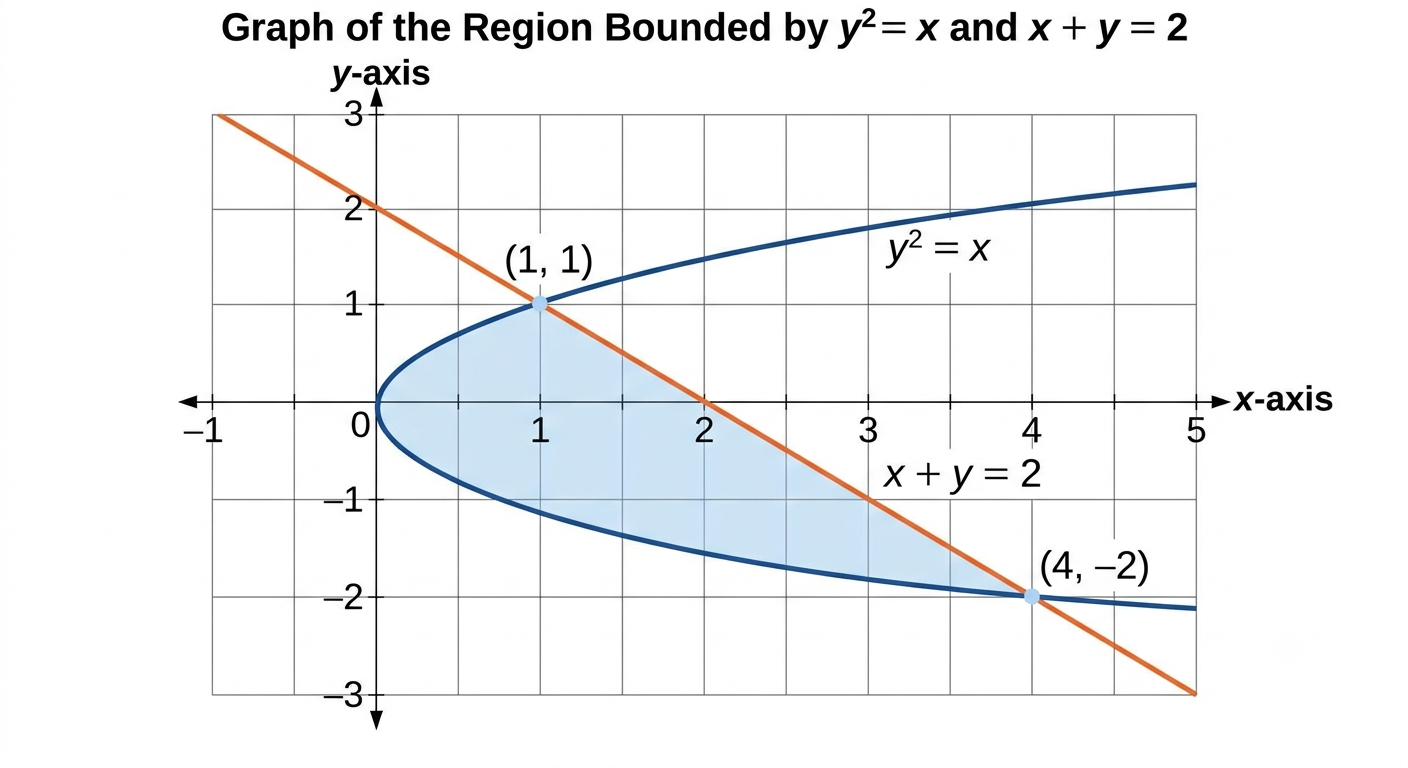
\includegraphics[width=0.5\textwidth]{figs/quad_plot.png}
 	\caption{Graph of Intersection }
 	\label{quad_plot.png}
 \end{figure} \newpage
 \begin{lstlisting}
      /codes/q26.py
 \end{lstlisting}
 
 
 %============Q28====================
 \item Evaluate:
 $$\int_0^{\pi} \frac{x \sin x}{1 + \cos^2 x} \, dx$$\\
 \solution
 From \eqref{king_prop}
 \begin{align}
 	I = \int_0^{\pi} \frac{\brak{\pi - x} \sin\brak{\pi - x}}{1 + \cos^2\brak{\pi - x}} \, dx
 	\label{eq:EE26BTECH11202-reflection_step}
 \end{align}
 \begin{align}
 	 = \int_0^{\pi} \frac{\brak{\pi - x} \sin x}{1 + \cos^2 x} \, dx
 	\label{eq:EE26BTECH11202-reflected_integral}
 \end{align}
 \begin{align}
 	I &= \pi \int_0^{\pi} \frac{\sin x}{1 + \cos^2 x} \, dx - \int_0^{\pi} \frac{x \sin x}{1 + \cos^2 x} \, dx
 \end{align}
 \begin{align}
 	I &= \pi \int_0^{\pi} \frac{\sin x}{1 + \cos^2 x} \, dx - I
 	\\
 	\implies 2I &= \pi \int_0^{\pi} \frac{\sin x}{1 + \cos^2 x} \, dx
 	\label{eq:EE26BTECH11202-combined_integral}
 \end{align}
 \begin{align}
 	u = \cos x \implies du = -\sin x \, dx \implies \sin x \, dx = -du 
 	\end{align}
 	\begin{align}
 	\brak{x = 0}:u = \cos 0 = 1 \quad \brak{x = \pi}: u = \cos \pi = -1
 \end{align}
 Substituting $u$ and $du$ 
 \begin{align}
 	2I &= \pi \int_{1}^{-1} \frac{-du}{1 + u^2}
 	\\
 	&= \pi \int_{-1}^{1} \frac{du}{1 + u^2}
 	\label{eq:EE26BTECH11202-u_integral}
 \end{align}
 From \eqref{king_prop}
 \begin{align}
 	2I &= 2\pi \int_{0}^{1} \frac{du}{1 + u^2}
 	\\
 	\implies I &= \pi \int_{0}^{1} \frac{du}{1 + u^2}
 \end{align}
 From \eqref{eq:intan}
 \begin{align}
 	I &= \pi \brak{\tan^{-1} u}_0^1
 	\\
 	&= \pi \brak{\tan^{-1}\brak{1} - \tan^{-1}\brak{0}}
 \end{align}
 \begin{align}
 	I = \pi \brak{\frac{\pi}{4} - 0} = \frac{\pi^2}{4}
 \end{align}
 
 %============Q29===================
 \item Using matrices, solve the following system of equations:
 \begin{align*} x + y + z &= 6 \\  x + 2z &= 7 \\  3x + y + z &= 12 \end{align*}
 \solution
 Expressing the system in  $\mathbf{A} \vec{x} = \vec{b}$:
 \begin{align}
 	\myvec{1 & 1 & 1 \\ 1 & 0 & 2 \\ 3 & 1 & 1} \myvec{x \\ y \\ z} = \myvec{6 \\ 7 \\ 12}
 \end{align}
 \begin{align}
 	\mathbf{M} = \myvec{1 & 1 & 1 & \vline & 6 \\ 1 & 0 & 2 & \vline & 7 \\ 3 & 1 & 1 & \vline & 12} \xrightarrow[R_2 \to R_2 - R_1]{R_3 \to R_3 - 3R_1}\myvec{1 & 1 & 1 & \vline & 6 \\ 0 & -1 & 1 & \vline & 1 \\ 0 & -2 & -2 & \vline & -6} 
 \end{align}
 \begin{align}
 \myvec{1 & 1 & 1 & \vline & 6 \\ 0 & -1 & 1 & \vline & 1 \\ 0 & -2 & -2 & \vline & -6} 	\xrightarrow{R_2 \to -R_2} \myvec{1 & 1 & 1 & \vline & 6 \\ 0 & 1 & -1 & \vline & -1 \\ 0 & -2 & -2 & \vline & -6} \\ \xrightarrow[R_3 \to -\frac{1}{4}R_3]{R_3 \to R_3 + 2R_2} \myvec{1 & 1 & 1 & \vline & 6 \\ 0 & 1 & -1 & \vline & -1 \\ 0 & 0 & 1 & \vline & 2}
 	\end{align}
 \begin{align}
 	\xrightarrow[R_2 \to R_2 + R_3]{R_1 \to R_1 - R_3}\myvec{1 & 1 & 0 & \vline & 4 \\ 0 & 1 & 0 & \vline & 1 \\ 0 & 0 & 1 & \vline & 2}
 	\end{align}
 	\begin{align}
 	x= 3,
 	y= 1,
 	z= 2
 	\end{align}
 	\begin{lstlisting}
 		/codes/q28.py
 	\end{lstlisting}
 	\begin{figure}[htbp] % [htbp] specifies preferred placement (here, top, bottom, page)
 		\centering
 		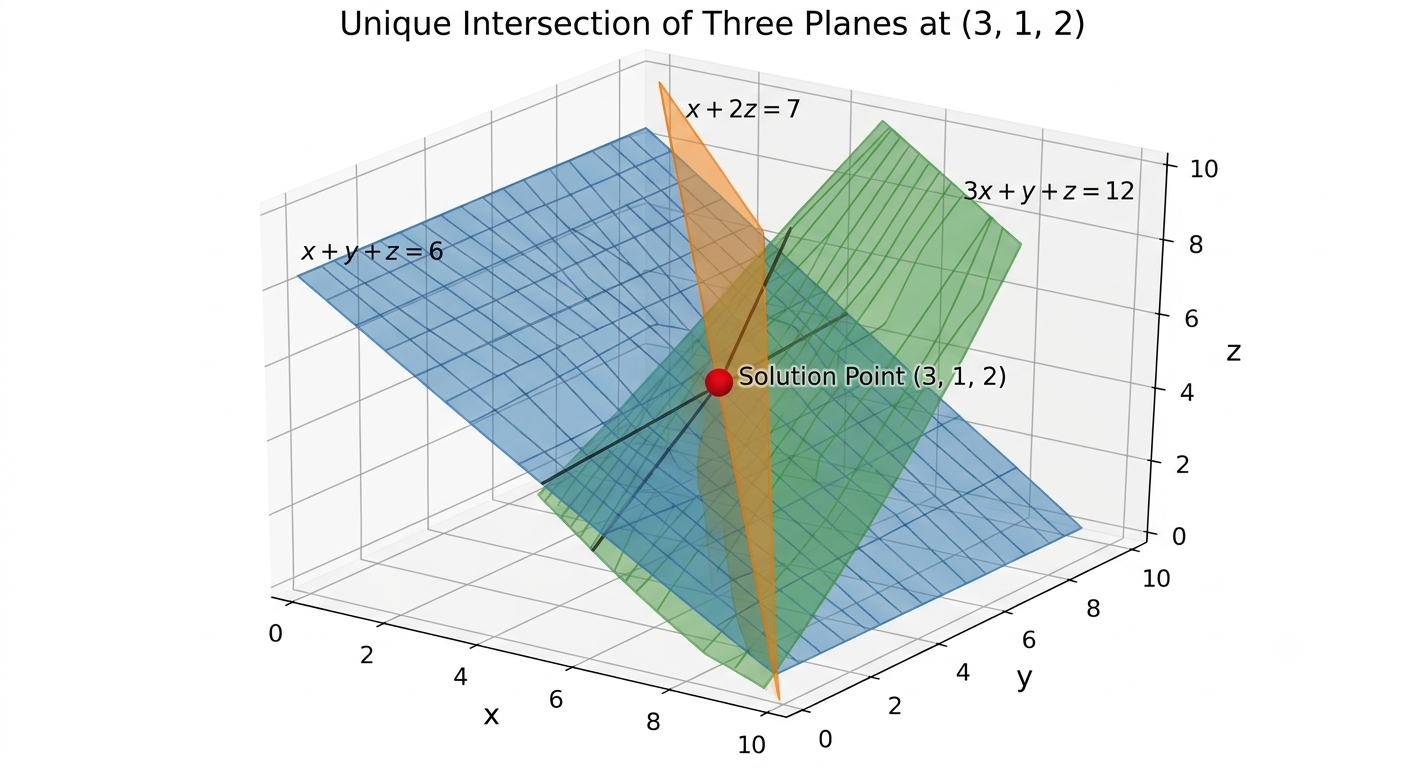
\includegraphics[width=0.5\textwidth]{figs/3D_plot.png}
 		\caption{Graph of Intersection }
 		\label{quad_plo.png}
 	\end{figure}
 	
 	
 %===========Q30======================
 \item Obtain the inverse of the matrix A=\myvec{2 & 0 & -1 \\
                                                 5 & 1 & 0 \\
                                                 0 & 1 & 3 \\} using elementary row operations.
                                                 \solution
  Constructing the augmented matrix $\brak{\mathbf{A} \mid \mathbf{I}_3}$ and performing elementary row operations reduces the system to $\brak{\mathbf{I}_3 \mid \mathbf{A}^{-1}}$ and as
 $\mydet{\vec{A}} = 1 \neq 0$
 \begin{align}
 	\mathbf{M} = \myvec{2 & 0 & -1 & \vline & 1 & 0 & 0 \\ 5 & 1 & 0 & \vline & 0 & 1 & 0 \\ 0 & 1 & 3 & \vline & 0 & 0 & 1}
 	\label{eq:EE26BTECH11202-aug_matrix}
 \end{align}
 \begin{align}
 	 \myvec{2 & 0 & -1 & \vline & 1 & 0 & 0 \\ 5 & 1 & 0 & \vline & 0 & 1 & 0 \\ 0 & 1 & 3 & \vline & 0 & 0 & 1} \xrightarrow[R_1 \leftrightarrow R_2]{R_2 \to R_2 - 2R_1} \myvec{1 & 1 & 2 & \vline & -2 & 1 & 0 \\ 2 & 0 & -1 & \vline & 1 & 0 & 0 \\ 0 & 1 & 3 & \vline & 0 & 0 & 1}
 	\end{align}
 	\begin{align}
 	\xrightarrow[R_2 \leftrightarrow R_3]{R_2 \to R_2 - 2R_1}	\myvec{1 & 1 & 2 & \vline & -2 & 1 & 0 \\ 0 & 1 & 3 & \vline & 0 & 0 & 1 \\ 0 & -2 & -5 & \vline & 5 & -2 & 0} \\
 	\xrightarrow{R_3 \to R_3 + 2R_2} \myvec{1 & 1 & 2 & \vline & -2 & 1 & 0 \\ 0 & 1 & 3 & \vline & 0 & 0 & 1 \\ 0 & 0 & 1 & \vline & 5 & -2 & 2}\\
 	\xrightarrow[R_1 \to R_1 - 2R_3]{R_2 \to R_2 - 3R_3}\myvec{1 & 1 & 0 & \vline & -12 & 5 & -4 \\ 0 & 1 & 0 & \vline & -15 & 6 & -5 \\ 0 & 0 & 1 & \vline & 5 & -2 & 2}
 		\end{align}
 		\begin{align}
 	\xrightarrow{R_1 \to R_1 - R_2}	\myvec{1 & 0 & 0 & \vline & 3 & -1 & 1 \\ 0 & 1 & 0 & \vline & -15 & 6 & -5 \\ 0 & 0 & 1 & \vline & 5 & -2 & 2}	
 			\end{align}
 			\begin{align}
 				\mathbf{A}^{-1} = \myvec{3 & -1 & 1 \\ -15 & 6 & -5 \\ 5 & -2 & 2}
 			\end{align}
 %====================Q31===================
 \item Coloured balls are distributed in three bags as shown in the following table:$$\begin{array}{|c|c|c|} \hline \text{Bag} & \text{Black balls} & \text{Red balls} \\ \hline \text{I} & 1 & 3 \\ \text{II} & 2 & 1 \\ \text{III} & 4 & 3 \\ \hline \end{array}$$
 A bag is selected at random and then two balls are randomly drawn from the selected bag. They happen to be black and red. What is the probability that they came from bag I?\\
 \solution
 $E_1$, $E_2$, and $E_3$ denote the mutually exclusive and exhaustive events.$A$ denote the observed outcome event: \textit{"Drawing 1 Black ball and 1 Red ball"}.
 \begin{align}
 	P\brak{E_1} = P\brak{E_2} = P\brak{E_3} = \frac{1}{3}
 \end{align}
 For Bag I ($E_1$):
 \begin{align}
 	P\brak{A \mid E_1} = \frac{\binom{1}{1} \binom{3}{1}}{\binom{4}{2}} = \frac{1 \times 3}{6} = \frac{3}{6} = \frac{1}{2}
 \end{align}
 For Bag II ($E_2$):
 \begin{align}
 	P\brak{A \mid E_2} = \frac{\binom{2}{1} \binom{1}{1}}{\binom{3}{2}} = \frac{2 \times 1}{3} = \frac{2}{3}
 \end{align}
 For Bag III ($E_3$):
 \begin{align}
 	P\brak{A \mid E_3} = \frac{\binom{4}{1} \binom{3}{1}}{\binom{7}{2}} = \frac{4 \times 3}{21} = \frac{12}{21} = \frac{4}{7}
 \end{align}
 From \eqref{tot_prop}
 \begin{align}
 	P\brak{A} &= \frac{1}{3} \brak{\frac{1}{2}} + \frac{1}{3} \brak{\frac{2}{3}} + \frac{1}{3} \brak{\frac{4}{7}}
 	\\
 	&= \frac{1}{3} \brak{\frac{1}{2} + \frac{2}{3} + \frac{4}{7}}
 \end{align}
 \begin{align}
 	P\brak{A} = \frac{1}{3} \times \frac{73}{42} = \frac{73}{126}
 \end{align}
 From \eqref{bayer}
 \begin{align}
 	P\brak{E_1 \mid A}	&= \frac{\frac{1}{3} \times \frac{1}{2}}{\frac{73}{126}} = \frac{\frac{1}{6}}{\frac{73}{126}}
 	\\
 	&= \frac{1}{6} \times \frac{126}{73} = \frac{21}{73}
 \end{align}
 \begin{lstlisting}
 	\codes\q30.py
 	\end{lstlisting}
 
 %==================Q32==============
 \item A dealer wishes to purchase a number of fans and sewing machines. He has only Rs. 5,760 to invest and has a space for at most 20 items. A fan costs him Rs. 360 and a sewing machine Rs. 240. His expectation is that he can sell a fan at a profit of Rs. 22 and a sewing machine at a profit of Rs. 18. Assuming that he can sell all the items that he can buy, how should he invest his money in order to maximize the profit? Formulate this as a linear programming problem and solve it graphically.
 \solution
 Let 
 \begin{align}
 	x &= \text{number of fans purchased} \\
 	y &= \text{number of sewing machines purchased}
 \end{align}
 The profit earned on selling one fan is Rs.~$22$ and one sewing machine is Rs.~$18$. The objective function $Z$ to maximize total profit is:
 \begin{align}
 	\text{Maximize } Z = 22x + 18y
 	\label{eq:EE26BTECH11202-objective}
 \end{align}
 The total capital available is Rs.~$5,760$, with cost per fan of Rs.~$360$ and per sewing machine of Rs.~$240$:
 \begin{align}
 	360x + 240y &\le 5760 \implies   3x + 2y \le 48
 \end{align}
 The maximum storage capacity is $20$ items:
 \begin{align}
 	x + y &\le 20
 	\label{eq:EE26BTECH11202-space_constraint}
 \end{align}
 Since the number of items purchased cannot be negative:
 \begin{align}
 	x \ge 0, \quad y \ge 0
 	\label{eq:EE26BTECH11202-non_negativity}
 \end{align}
 \begin{align}
 	\text{Line 1 } (L_1): & \quad 3x + 2y = 48
 	\\
 	\text{Line 2 } (L_2): & \quad x + y = 20
 \end{align}
 \begin{align}
 	\text{For } x = 0: & \quad 2y = 48 \implies y = 24 \implies (0, 24)
 	\\
 	\text{For } y = 0: & \quad 3x = 48 \implies x = 16 \implies A(16, 0)
 \end{align}
 
 Intersections of $L_2$ with Axes:
 \begin{align}
 	\text{For } x = 0: & \quad y = 20 \implies C(0, 20)
 	\\
 	\text{For } y = 0: & \quad x = 20 \implies (20, 0)
 \end{align} 	
 Solving
 \begin{align}
 	\myvec{3 & 2 \\ 1 & 1} \myvec{x \\ y} = \myvec{48 \\ 20}
 \end{align}
 Subtracting $2 \times L_2$ from $L_1$:
 \begin{align}
 	\brak{3x + 2y} - 2\brak{x + y} = 48 - 2\brak{20} \implies x = 8
 \end{align}
 Substituting $x = 8$ into $L_2$:
 \begin{align}
 	8 + y = 20 \implies y = 12 \implies B(8, 12)
 \end{align}
 
 The maximum profit of Rs.~$392$ occurs uniquely at vertex $B(8, 12)$.
 \begin{align}
 	\text{Total Investment: } & 360(8) + 240(12) = 2880 + 2880 = \text{Rs. } 5760 \quad (\text{100\% capital utilized})
 	\\
 	\text{Total Items: } & 8 + 12 = 20 \quad (\text{100\% capacity utilized})
 \end{align}
 \begin{figure}[htbp] % [htbp] specifies preferred placement (here, top, bottom, page)
 	\centering
 	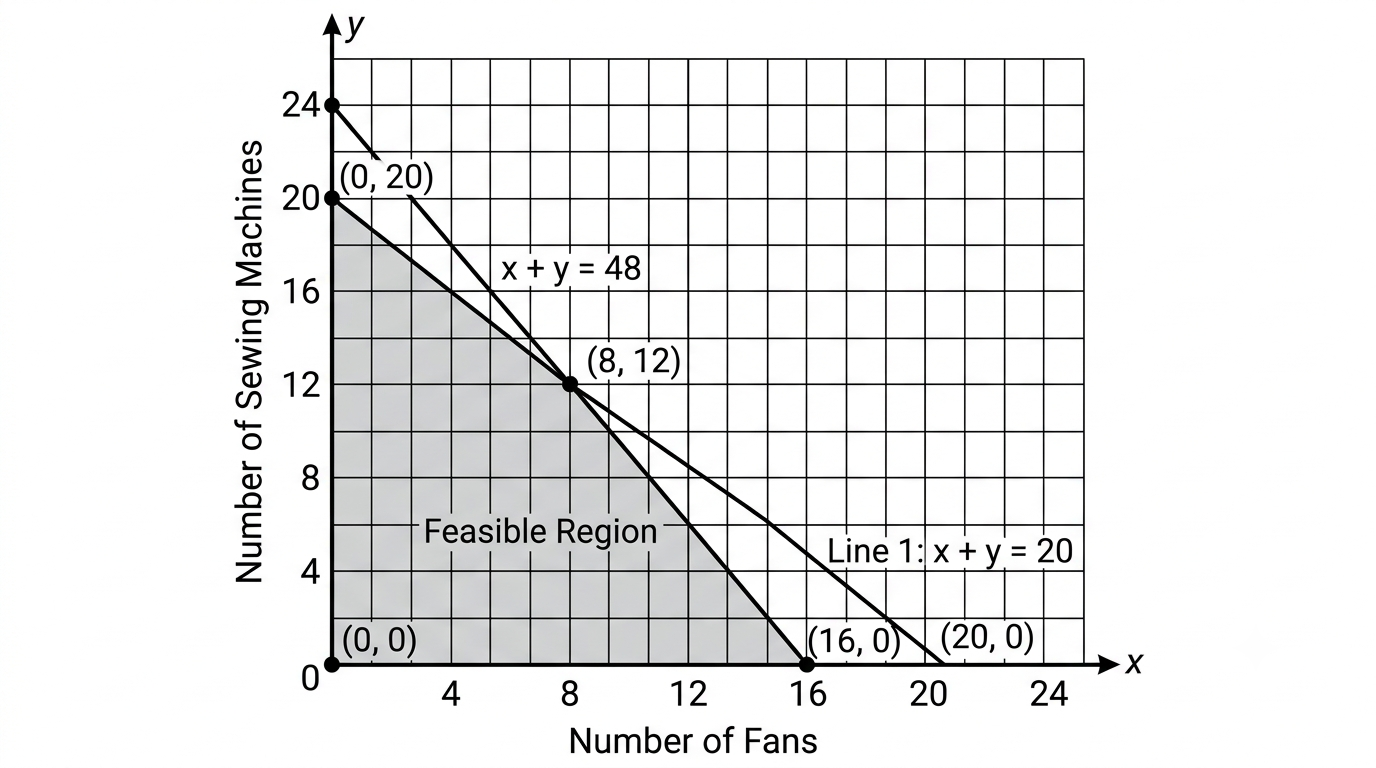
\includegraphics[width=0.5\textwidth]{figs/q31.png}
 	\caption{Graphical Representation}
 	\label{Graphical Representation.png}
 \end{figure}\newpage
 \begin{lstlisting}
 	/codes/q31.py
 \end{lstlisting}
 %===============Q33=================
 \item If the sum of the lengths of the hypotenuse and a side of a right-angled triangle is given, show that the area of the triangle is maximum when the angle between them is $\frac{\pi}{3}$.\\
 \solution
 \begin{align}
 	\text{Hypotenuse length} &= h
 	\\
 	\text{Base side length} &= x
 	\\
 	\text{Perpendicular height} &= y
 	\\
 	\text{Angle between base } x \text{ and hypotenuse } h &= \theta
 \end{align}
 \begin{align}
 	h + x = k \implies h = k - x
 	\label{eq:EE26BTECH11202-hyp_constraint}
 \end{align}
 \begin{align}
 	y &= \sqrt{h^2 - x^2} = \sqrt{\brak{k - x}^2 - x^2}
 	\\
 	&= \sqrt{k^2 - 2kx + x^2 - x^2} = \sqrt{k^2 - 2kx}
 	\label{eq:EE26BTECH11202-height_expr}
 \end{align}
 \begin{align}
 	A\brak{x} = \frac{1}{2} x y = \frac{1}{2} x \sqrt{k^2 - 2kx}
 \end{align}
 To simplify differentiation, define the auxiliary objective function $Z\brak{x} = \brak{A\brak{x}}^2$:
 \begin{align}
 	Z\brak{x} = \frac{1}{4} x^2 \brak{k^2 - 2kx} = \frac{1}{4} \brak{k^2 x^2 - 2k x^3}
 	\label{eq:EE26BTECH11202-squared_area}
 \end{align}
 Since $A\brak{x} > 0$, maximizing $Z\brak{x}$ is strictly equivalent to maximizing $A\brak{x}$.
 Differentiating 
 \begin{align}
 	\frac{dZ}{dx} &= \frac{1}{4} \frac{d}{dx} \brak{k^2 x^2 - 2k x^3}
 	\\
 	&= \frac{1}{4} \brak{2k^2 x - 6k x^2} = \frac{1}{2} k x \brak{k - 3x}
 	\label{eq:EE26BTECH11202-first_derivative}
 \end{align}
 Setting $\frac{dZ}{dx} = 0$ to locate critical points:
 \begin{align}
 	\frac{1}{2} k x \brak{k - 3x} = 0
 \end{align}
 \begin{align}
 	k - 3x = 0 \implies x = \frac{k}{3}
 	\label{eq:EE26BTECH11202-critical_x}
 \end{align}
 Differentiating \eqref{eq:EE26BTECH11202-first_derivative} with respect to $x$:
 \begin{align}
 	\frac{d^2 Z}{dx^2} = \frac{1}{4} \brak{2k^2 - 12kx}
 \end{align}
 
 Evaluating at the critical point $x = \frac{k}{3}$:
 \begin{align}
 	\mydet{\frac{d^2 Z}{dx^2}}_{x = \frac{k}{3}} &= \frac{1}{4} \brak{2k^2 - 12k \brak{\frac{k}{3}}}
 	\\
 	&= \frac{1}{4} \brak{2k^2 - 4k^2} = -\frac{k^2}{2} < 0
 \end{align}
 $Z\brak{x}$ (and hence area $A\brak{x}$) achieves a strict local maximum at $x = \frac{k}{3}$.
 \begin{align}
 	h = k - \frac{k}{3} = \frac{2k}{3}
 \end{align}
 \begin{align}
 	\cos \theta =\frac{x}{h} = \frac{\frac{k}{3}}{\frac{2k}{3}} = \frac{1}{2}
 \end{align}
 \begin{align}
 \theta = \cos^{-1}\brak{\frac{1}{2}} = \frac{\pi}{3}
 \end{align}
 %===============Q34=============
 
\end{enumerate}
